% Task C12
% Source volume: upper
% Physical scan pages: 392--419
% Printed book pages: 375--402
% Transcribe only source content; omit running headers, footers, and printed page numbers.
\chapter{广义积分}

% BEGIN TRANSCRIPTION
广义积分（也称反常积分）作为变限积分函数的极限，其许多性质与定积分类似。本章共分 5 节。§12.1 讨论广义积分的定义。§12.2 与 §12.3 分别讨论广义积分的敛散性判别与计算。§12.4 讨论无穷限广义积分的一些特殊性质。最后一节为学习要点和两组参考题。

广义积分与无穷级数之间有密切联系。在各种数学分析教材中两者的教学顺序并不相同。虽然本书在第二章中已经提到了无穷级数的概念（见 2.2.3 小节末的注解以及例题 2.2.6，2.2.9，命题 2.5.2 等），但是要到下册中才有关于无穷级数的全面论述。因此这方面的联系也要到后面介绍（例如下册命题 13.2.1 等）。

\section{广义积分的定义}

\subsection{基本定义}

\begin{enumerate}
  \item 在定积分一章中给出函数 $f$ 为 Riemann 可积的定义时，有两个基本限制：
  \begin{enumerate}[label=(\arabic*)]
    \item 积分区间 $[a,b]$ 必须有限，
    \item 函数 $f$ 在 $[a,b]$ 上必须有界。
  \end{enumerate}
  前者是在积分的分割定义中隐含的必要条件，后者则可以作为可积的必要条件而得到（见命题 10.1.1）。广义积分就是在这两个方面对于定积分定义的突破。今后也称原有的 Riemann 积分为常义积分。

  \item 为方便起见，引入如下定义：设 $I$ 为区间，函数 $f$ 在 $I$ 上有定义，如果对任意有界闭区间 $[a,b]\subseteq I$，$f\in R[a,b]$，则称 $f$ 在 $I$ 上内闭可积。

  \item 广义积分的定义方法是通过对常义积分取极限。称 $b$ 为函数 $f(x)$ 在定义域区间 $[a,b)$ 上的奇点，如果 $b=+\infty$ 或者 $f(x)$ 在点 $b$ 左侧邻近无界。假如 $f(x)$ 在区间 $[a,b)$ 上内闭可积，$b$ 为 $f(x)$ 在 $[a,b)$ 上的奇点，则定义广义积分
  \[
    \int_a^b f=\int_a^b f(x)\,\dd x=\lim_{b'\to b-}\int_a^{b'}f(x)\,\dd x.
  \]
  如果上式右边极限存在且有限（在 $b=+\infty$ 时，$b'\to b-$ 是指 $b'\to+\infty$），则称广义积分 $\int_a^b f$ 收敛或 $f$ 广义可积（在不产生混淆时也可简称可积）；否则，称广义积分 $\int_a^b f$ 发散或 $f$ 广义不可积（简称不可积）。类似地，定义以 $a$ 为奇点的广义积分 $\int_a^b f$ 及其敛散性。

  \item 称广义积分 $\int_a^b f$ 绝对收敛或 $f$（广义）绝对可积，若广义积分 $\int_a^b\abs{f}$ 收敛。

  \item 设 $b$ 为 $f$ 在 $[a,b)$ 上的奇点。如果 $b=+\infty$，则称广义积分 $\int_0^{+\infty}f$ 为无穷限广义积分，简称为无穷限积分或无穷积分。如果 $b$ 为有限数，则称广义积分 $\int_a^b f$ 为无界广义积分，简称为无界积分或瑕积分，也称奇点 $b$ 为瑕点。这两类广义积分不但往往可以用换元法互换，而且它们的定义与很多性质也可以统一叙述。

  \item 设 $a<c<b$，如果 $c$ 为 $f$ 在 $[a,c)$ 与 $(c,b]$ 上的奇点或 $a,b$ 分别为 $f$ 在 $(a,c]$ 与 $[c,b)$ 上的奇点，则定义广义积分
  \[
    \int_a^b f=\int_a^c f+\int_c^b f,
  \]
  当右边两个广义积分都收敛时，称广义积分 $\int_a^b f$ 收敛；否则，称广义积分 $\int_a^b f$ 发散。
\end{enumerate}

\begin{xremark}
\textbf{1}\quad 上述无穷限积分与无界积分的统一叙述可以简化广义积分的许多结果的表达。但两类广义积分毕竟还有区别（例如见 §12.4），学习本章时要注意两类广义积分的异同。
\end{xremark}

\begin{xremark}
\textbf{2}\quad 对不定积分、定积分和广义积分，可积的含义是不同的。不定积分的可积是指其有初等函数族，定积分的可积是指其 Riemann 可积，即 Riemann 积分存在，而广义积分可积是指广义积分收敛。这似乎容易引起混淆，但在上下文不会引起混淆的情况下，使用可积这个术语可以简化叙述。
\end{xremark}

除了以上基本概念之外，还需要知道广义积分的主值。以下对两种广义积分分别给出它们的主值定义。

设函数 $f$ 在 $(-\infty,+\infty)$ 上内闭可积，定义
\[
  \mathrm{P.V.}\int_{-\infty}^{+\infty}f=\lim_{A\to+\infty}\int_{-A}^{A}f
\]
为广义积分 $\int_{-\infty}^{+\infty}f$ 的 Cauchy 主值，如果右边极限存在的话。

对于无界积分，设 $f$ 在区间 $[a,b]$ 中只有一个瑕点 $c$，$a<c<b$，则定义
\[
  \mathrm{P.V.}\int_a^b f=\lim_{\delta\to0+}\left(\int_a^{c-\delta}f+\int_{c+\delta}^bf\right)
\]
为广义积分 $\int_a^b f$ 的 Cauchy 主值，如果右边极限存在的话。

容易看出，若广义积分收敛，则其主值与广义积分的值相同；但是当广义积分发散时，它的主值仍可能存在。因此主值是广义积分概念的一个推广，它在理论和应用上都很有价值。对于本章内容来说，如果事先能判定某个广义积分收敛，则在计算该广义积分时可以用主值来代替，这有时会带来方便。

\subsection{广义积分与和式极限}

虽然广义积分是通过对常义积分取极限得到，但在被积函数单调情况下也有可能如常义积分那样直接从积分和式取极限得到。首先我们讨论有界区间上的无界广义积分。下面就是这类结果之一。

\begin{xexample}[12.1.1]
设 $f$ 在 $(0,1)$ 上单调，无界广义积分 $\int_0^1 f(x)\,\dd x$ 收敛，则有
\begin{equation}
  \lim_{n\to\infty}\frac{f\left(\frac1n\right)+f\left(\frac2n\right)+\cdots+f\left(\frac{n-1}{n}\right)}{n}=\int_0^1 f(x)\,\dd x.
  \tag{12.1}
  \label{eq:12.1}
\end{equation}
\end{xexample}
\begin{xproof}
不妨只讨论 $f$ 单调增加，则有不等式
\[
  \int_0^{1-\frac1n}f(x)\,\dd x
  \leq
  \frac{f\left(\frac1n\right)+f\left(\frac2n\right)+\cdots+f\left(\frac{n-1}{n}\right)}{n}
  \leq
  \int_{\frac1n}^1 f(x)\,\dd x.
\]
这两边的积分中至少有一个是广义积分。然后令 $n\to\infty$ 即可。
\end{xproof}

\begin{xremark}
这里有几点需要注意。首先，单调性条件只要在奇点邻近满足即可。其次，在只有一个奇点的情况，从等式 (12.1) 左边极限存在可推出右边的广义积分收敛。然而对于有两个奇点的情况这是不成立的。例如
\[
  f(x)=\frac1x-\frac1{1-x}
\]
就是如此（见 [48] 第一卷 253 页）。
\end{xremark}

对于无穷限广义积分也有类似结果。但是这时的积分和式本身已经是无穷项求和，也就是无穷级数。在学习无穷级数理论之前，可以先按照 2.2.3 小节末的注解来理解。

\begin{xexample}[12.1.2]
设 $f$ 在 $[0,+\infty)$ 上单调，$\int_0^{+\infty} f(x)\,\dd x$ 收敛，则有
\[
  \lim_{h\to0+}h\sum_{n=1}^{\infty}f(nh)=\int_0^{+\infty}f(x)\,\dd x.
\]
\end{xexample}
\begin{xproof}
不妨假定 $f$ 单调减少。首先可以证明 $f$ 在 $[0,+\infty)$ 上非负。用反证法：如果在某点 $x_0$ 处有 $f(x_0)<0$，则就有
\[
  \int_{x_0}^A f(x)\,\dd x\leq f(x_0)(A-x_0)\to-\infty\qquad(A\to+\infty),
\]
这与无穷限广义积分收敛的条件矛盾。

于是，对任意正整数 $n$，我们有
\[
  \int_h^{(n+1)h}f(x)\,\dd x
  \leq \sum_{k=1}^n hf(kh)
  =h\sum_{k=1}^n f(kh)
  \leq \int_0^{nh}f(x)\,\dd x.
\]
注意到中间的和式作为 $n$ 的函数（即数列）为单调增加，且有上界，因此存在极限。令 $n\to+\infty$，得到
\[
  \int_h^{+\infty}f(x)\,\dd x
  \leq h\sum_{n=1}^{\infty}f(nh)
  \leq \int_0^{+\infty}f(x)\,\dd x.
\]
再令 $h\to0+$ 即得所要求证的结果。
\end{xproof}

\subsection{练习题}

\begin{xexercise}[1]
设 $f$ 在 $[0,+\infty)$ 上非负连续，且积分 $\int_0^{+\infty}f=0$，证明：$f\equiv0$。
\end{xexercise}
\begin{xsolution}
设存在 $x_0\geq0$ 使 $f(x_0)>0$。由连续性，存在 $\delta>0$ 与 $c>0$，使得在
$[0,+\infty)\cap(x_0-\delta,x_0+\delta)$ 上有 $f(x)\geq c$。于是该小区间上的积分严格为正，而 $f\geq0$，故
\[
  \int_0^{+\infty}f(x)\,\dd x>0,
\]
与已知矛盾。因此任意 $x\geq0$ 都有 $f(x)=0$，即 $f\equiv0$。
\end{xsolution}


\begin{xexercise}[2]
如果广义积分 $\int_a^b f^2$ 收敛，则称 $f$ 在 $[a,b]$ 上平方可积。分无穷限积分与无界积分两种情况讨论广义积分的平方可积性与绝对可积性之间的关系。
\end{xexercise}
\begin{xsolution}
先讨论无穷限积分。平方可积与绝对可积一般互不推出。比如在 $[1,+\infty)$ 上
\[
  f(x)=x^{-3/4}
\]
满足 $\int_1^{+\infty}f^2<+\infty$，但 $\int_1^{+\infty}|f|=+\infty$，所以平方可积不推出绝对可积。

反过来，取在每个区间 $[n,n+1]$ 内的连续三角形尖峰 $f_n$，其高为 $n^2$、底宽为 $2n^{-5}$，且不同尖峰支集互不相交；令 $f$ 为这些尖峰之和。则
\[
  \int_1^{+\infty}|f(x)|\,\dd x
  =\sum_{n=1}^{\infty}\frac12(2n^{-5})n^2
  =\sum_{n=1}^{\infty}\frac1{n^3}<+\infty,
\]
而一个高为 $H$、底宽为 $2w$ 的三角形平方积分为 $2H^2w/3$，故
\[
  \int_1^{+\infty}f^2(x)\,\dd x
  =\frac23\sum_{n=1}^{\infty}n^4n^{-5}
  =\frac23\sum_{n=1}^{\infty}\frac1n=+\infty.
\]
所以绝对可积也不推出平方可积。

对有限区间上的无界积分，情况不同。若 $f$ 在 $[a,b]$ 上平方可积，则对避开瑕点的任意有限子区间应用 Cauchy--Schwarz 不等式，并令端点趋于瑕点，得到
\[
  \int_a^b|f(x)|\,\dd x
  \leq \sqrt{b-a}\left(\int_a^b f^2(x)\,\dd x\right)^{1/2}<+\infty.
\]
故平方可积必绝对可积。逆命题不成立，例如在 $(0,1]$ 上 $f(x)=x^{-2/3}$ 绝对可积，而 $f^2(x)=x^{-4/3}$ 不可积。
\end{xsolution}


\begin{xexercise}[3]
设 $f\in C(0,1]$，$f(0+)=+\infty$，定义函数 $f_n(x)=\min\{f(x),n\}$，$0<x\leq1$，$n\in\NN_+$。证明：广义积分 $\int_0^1f$ 收敛的充分必要条件是存在有限极限
  \[
    \lim_{n\to\infty}\int_0^1 f_n(x)\,\dd x.
  \]
\end{xexercise}
\begin{xsolution}
由 $f(0+)=+\infty$，可取 $c\in(0,1)$，使 $f(x)>0$ 对 $0<x\leq c$ 成立。又因为 $f_n(x)=\min\{f(x),n\}$ 随 $n$ 单调增加。

若 $\int_0^1f$ 收敛，则对任意固定 $\varepsilon\in(0,c)$，当 $n$ 足够大时，$f_n=f$ 在 $[\varepsilon,1]$ 上成立，于是
\[
  \int_\varepsilon^1f(x)\,\dd x
  \leq \liminf_{n\to\infty}\int_0^1 f_n(x)\,\dd x.
\]
另一方面，在 $(0,c]$ 上有 $0\leq f_n\leq f$，而 $[c,1]$ 上当 $n$ 足够大时 $f_n=f$，故
\[
  \int_0^1 f_n(x)\,\dd x\leq \int_0^1 f(x)\,\dd x
\]
对充分大的 $n$ 成立。令 $\varepsilon\to0+$ 可知
\[
  \lim_{n\to\infty}\int_0^1f_n(x)\,\dd x=\int_0^1f(x)\,\dd x.
\]

反之，设左边极限为有限数 $L$。当 $n$ 足够大时，$f_n=f$ 在 $[c,1]$ 上成立，于是
\[
  \int_0^c f_n(x)\,\dd x
  =\int_0^1f_n(x)\,\dd x-\int_c^1f(x)\,\dd x
\]
有统一上界。对任意 $\varepsilon\in(0,c)$，再取 $n$ 足够大使 $f_n=f$ 于 $[\varepsilon,c]$，则
\[
  0\leq\int_\varepsilon^c f(x)\,\dd x
  \leq\int_0^c f_n(x)\,\dd x.
\]
因此 $\int_\varepsilon^c f$ 在 $\varepsilon\to0+$ 时单调有界，极限存在且有限，故 $\int_0^1f$ 收敛。
\end{xsolution}


\begin{xexercise}[4]
设 $f$ 在 $(-\infty,+\infty)$ 上内闭可积，$\int_{-\infty}^{+\infty}f^2$ 收敛，证明：对于任何实数 $a$，下列广义积分也收敛：
  \[
    \int_{-\infty}^{+\infty}\abs{f(x)f(x+a)}\,\dd x.
  \]
\end{xexercise}
\begin{xsolution}
由
\[
  2|uv|\leq u^2+v^2
\]
有
\[
  |f(x)f(x+a)|\leq\frac12\bigl(f^2(x)+f^2(x+a)\bigr).
\]
积分并作平移换元，得到
\[
  \int_{-\infty}^{+\infty}|f(x)f(x+a)|\,\dd x
  \leq\frac12\int_{-\infty}^{+\infty}f^2(x)\,\dd x
  +\frac12\int_{-\infty}^{+\infty}f^2(x+a)\,\dd x
  =\int_{-\infty}^{+\infty}f^2(x)\,\dd x<+\infty.
\]
所以所给广义积分绝对收敛。
\end{xsolution}


\begin{xexercise}[5]
设 $f$ 在 $(-\infty,+\infty)$ 上内闭可积，并且 $\lim_{x\to+\infty}f(x)=A$，$\lim_{x\to-\infty}f(x)=B$ 都存在且有限。证明：对任意实数 $a>0$，广义积分
  \[
    \int_{-\infty}^{+\infty}[f(x+a)-f(x)]\,\dd x
  \]
  收敛，并求它的值。
\end{xexercise}
\begin{xsolution}
先取 $M,N>0$。换元后
\begin{align*}
  \int_{-M}^{N}[f(x+a)-f(x)]\,\dd x
  &=\int_{N}^{N+a}f(t)\,\dd t-\int_{-M}^{-M+a}f(t)\,\dd t.
\end{align*}
当 $N\to+\infty$ 时，由 $f(t)\to A$，第一项趋于 $aA$；当 $M\to+\infty$ 时，由 $f(t)\to B$，第二项趋于 $aB$。因此两侧无穷限积分分别存在，且
\[
  \int_{-\infty}^{+\infty}[f(x+a)-f(x)]\,\dd x=a(A-B).
\]
\end{xsolution}


\begin{xexercise}[6]
找出以下广义积分计算中的错误，说明理由，并计算其主值。在积分
  \[
    \int_{-\frac12}^{\frac12}\frac{\dd x}{x\sqrt{1-x^2}}
  \]
  中，由于被积函数是奇函数，积分区间关于原点对称，从而所求积分为 0。
\end{xexercise}
\begin{xsolution}
错误在于 $x=0$ 是瑕点，广义积分必须拆成
\[
  \int_{-1/2}^{0}\frac{\dd x}{x\sqrt{1-x^2}}
  +\int_{0}^{1/2}\frac{\dd x}{x\sqrt{1-x^2}},
\]
而不能利用对称性把两个发散量相消。作 $x=\sin t$，有
\[
  \int\frac{\dd x}{x\sqrt{1-x^2}}=\int\csc t\,\dd t
  =\ln\left|\tan\frac t2\right|+C.
\]
故左侧积分趋于 $-\infty$，右侧积分趋于 $+\infty$，原广义积分发散。但其 Cauchy 主值为
\[
  \operatorname{P.V.}\int_{-1/2}^{1/2}\frac{\dd x}{x\sqrt{1-x^2}}
  =\lim_{\varepsilon\to0+}
  \left(\int_{-1/2}^{-\varepsilon}+\int_{\varepsilon}^{1/2}\right)
  \frac{\dd x}{x\sqrt{1-x^2}}=0,
\]
因为被积函数为奇函数且截去区间关于原点对称。
\end{xsolution}


\section{广义积分的敛散性判别法}

本节在第一小节中从一个例题开始，讨论敛散性判别法。对 Dirichlet 判别法和 Abel 判别法的必要性给出证明和改进。在后两个小节中给出例题和练习题。

\subsection{敛散性判别法}

下面先看一个简单例题。在其中我们将从基本定义出发进行讨论，而不直接应用某个判别法，其目的是说明这里所遇到的问题的一般特征。

\begin{xexample}[12.2.1]
设 $f$ 在 $[a,+\infty)$（$a>1$）上内闭可积，且已知广义积分
\[
  \int_a^{+\infty}x f(x)\,\dd x
\]
收敛，证明：广义积分 $\int_a^{+\infty}f(x)\,\dd x$ 也收敛。
\end{xexample}
\begin{xproof}
如果 $f$ 非负，则可以写出不等式
\[
  0\leq\int_a^A f(x)\,\dd x\leq\int_a^A x f(x)\,\dd x,
\]
其中两个积分作为变上限 $A$ 的函数都是单调增加函数。由于右边在 $A\to+\infty$ 时存在极限，中间的积分作为 $A\in[a,+\infty)$ 的函数就是有上界的单调增加函数，因此当 $A\to+\infty$ 时也有极限。这就证明了 $f$ 在区间 $[a,+\infty)$ 上的广义积分收敛。对于 $f$ 非正情况的讨论是类似的。这就是比较判别法。

但是当 $f$ 为变号函数时，上面的比较方法不能直接使用。\footnote{如果 $f$ 绝对可积，则比较方法还可以用。} 这时需要两个新的工具：（1）广义积分的 Cauchy 收敛准则；（2）积分第二中值定理。

任取 $a<A<A'$，对于积分
\[
  \abs*{\int_A^{A'}f(x)\,\dd x}
  =\abs*{\int_A^{A'}xf(x)\cdot\frac1x\,\dd x},
\]
利用右边积分号下第二个因子 $1/x$ 单调且非负，就有 $\xi\in(A,A')$，使得成立
\[
  \abs*{\int_A^{A'}f(x)\,\dd x}
  =\abs*{\frac1A\int_A^\xi x f(x)\,\dd x},
\]
然后利用条件就可以使得左边的积分当 $A,A'$ 充分大时小于事先给定的 $\varepsilon>0$，因此 $f$ 在 $[a,+\infty)$ 上广义可积。
\end{xproof}

\begin{xremark}
\textbf{1}\quad 注意在证明过程中两次应用 Cauchy 收敛准则，一次是用收敛的必要条件，另一次是用收敛的充分条件。实际上从广义积分开始，在后面的无穷级数和含参积分各章中各种形式的 Cauchy 收敛准则都要起非常重要的作用。其中的基本理由和上面这个简单例题是相同的。初学者可以复习一下 §3.4 中对于 Cauchy 收敛准则的基本内容。
\end{xremark}

\begin{xremark}
\textbf{2}\quad 上面的证明实际上重复了 Abel 判别法与 Dirichlet 判别法的推导过程。当然可以直接应用这两个判别法之一来达到目的。

这里需要指出，Abel 判别法和 Dirichlet 判别法中的条件不仅是广义积分收敛的充分条件，同时也是必要条件。当然，Abel 判别法的必要性是平凡的。但是 Dirichlet 判别法的必要性则是较新的发现，多数教科书中都没有收入。下面我们给出它的证明（参见 [68]）。
\end{xremark}

\begin{xproposition}[12.2.1（Dirichlet 判别法）]
设 $f$ 在 $[a,b)$ 上内闭可积，$b$ 为奇点，广义积分 $\int_a^b f$ 收敛的充分必要条件是存在分解 $f=uv$，使得
\begin{enumerate}[label=(\arabic*)]
  \item 函数 $u$ 在 $[a,b)$ 上单调，且 $\lim_{x\to b}u(x)=0$；
  \item 对任何 $b'>a$，积分 $\int_a^{b'}v(x)\,\dd x$ 存在且有界。
\end{enumerate}
\end{xproposition}
\begin{xproof}
充分性见一般教科书。下面只对 $b=+\infty$ 情况的必要性给出证明，对于其他情况的证明是类似的。

由于广义积分 $\int_a^{+\infty}f(x)\,\dd x$ 收敛，根据 Cauchy 收敛准则，存在 $A_1>a$，使得对于任何 $B>A\geq A_1$，成立
\[
  \abs*{\int_A^B f(x)\,\dd x}<1.
\]
归纳地可知，对于 $n\geq2$，存在 $A_n>A_{n-1}+1$，使得对于任何 $B>A\geq A_n$，成立
\[
  \abs*{\int_A^B f(x)\,\dd x}<\frac1{n^3}.
\]
这样得到的 $\{A_n\}$ 是严格单调增加的无穷大数列。

现在定义
\begin{equation}
  u(x)=
  \begin{cases}
    1, & a\leq x\leq A_1,\\
    \dfrac1n, & A_n<x\leq A_{n+1},\ n\in\NN_+,
  \end{cases}
  \tag{12.2}
  \label{eq:12.2}
\end{equation}
和
\begin{equation}
  v(x)=\frac{f(x)}{u(x)},\qquad a\leq x<+\infty.
  \tag{12.3}
  \label{eq:12.3}
\end{equation}
这样就有分解 $f=uv$，其中函数 $u$ 满足条件 (1) 是明显的，下面只需验证函数 $v$ 满足条件 (2)。容易看出 $v$ 在 $[a,+\infty)$ 上内闭可积，因此只需要证明它在任何区间 $[a,A]$ 上的积分有界。

由于当 $a\leq A\leq A_1$ 时 $v(x)=f(x)$，因此存在常数 $L>0$，使得对这样的 $A$ 成立
\[
  \abs*{\int_a^A v(x)\,\dd x}<L.
\]
若 $A>A_1$，则存在 $n$，使得 $A_n<A\leq A_{n+1}$。这时根据定义 (12.3) 和 (12.2)，可以先作分解：
\[
  \int_a^A v(x)\,\dd x
  =\left[\int_a^{A_1}+\int_{A_1}^{A_2}+2\int_{A_2}^{A_3}+\cdots+(n-1)\int_{A_{n-1}}^{A_n}+n\int_{A_n}^A\right]f(x)\,\dd x,
\]
然后就不难作出所需要的估计如下：
\begin{align*}
  \abs*{\int_a^A v(x)\,\dd x}
  &\leq \abs*{\int_a^{A_1}f}
   +\abs*{\int_{A_1}^{A_2}f}
   +2\abs*{\int_{A_2}^{A_3}f}+\cdots
   +(n-1)\abs*{\int_{A_{n-1}}^{A_n}f}
   +n\abs*{\int_{A_n}^Af}\\
  &\leq L+1+2\cdot\frac1{2^3}+\cdots+(n-1)\cdot\frac1{(n-1)^3}+n\cdot\frac1{n^3}\\
  &=L+1+\frac1{2^2}+\cdots+\frac1{n^2}\\
  &<L+1+\frac1{1\cdot2}+\cdots+\frac1{(n-1)n}<L+2.
\end{align*}
\end{xproof}

下面我们再观察 Abel 判别法。

\begin{xproposition}[12.2.2（Abel 判别法）]
设 $f$ 在 $[a,b)$ 上内闭可积，$b$ 为奇点，广义积分 $\int_a^b f$ 收敛的充分必要条件是存在分解 $f=uv$，使得
\begin{enumerate}[label=(\arabic*)]
  \item 函数 $u$ 在 $[a,b)$ 上单调有界；
  \item 积分 $\int_a^b v(x)\,\dd x$ 收敛。
\end{enumerate}
\end{xproposition}

众所周知，Abel 判别法的充分性可以从 Dirichlet 判别法导出，同时其必要性是平凡的，因为可以令 $u=1,v=f$。但是应用 Dirichlet 判别法的必要性可以证明，在 Abel 判别法中的必要性可以加强为：$u(x)$ 不仅单调，而且 $u(b-)=0$（见 [68]）。

证明是简单的。设 $f=uv$ 是满足 Dirichlet 判别法条件的分解。不妨设其中 $u$ 非负。然后令
\[
  u_1=\sqrt{u},\qquad v_1=\sqrt{u}v,
\]
就不难看出 $f=u_1v_1$ 是满足 Abel 判别法条件的分解，而且 $u_1(b-)=0$。

\subsection{例题}

\begin{xexample}[12.2.2]
讨论下列广义积分的敛散性：
\begin{enumerate}[label=(\arabic*)]
  \item $\displaystyle\int_1^{+\infty}\left(\frac{x}{x^2+p}-\frac{p}{x+1}\right)\,\dd x$；
  \item $\displaystyle\int_0^1\abs{\ln x}^p\,\dd x$；
  \item $\displaystyle\int_0^{+\infty}\frac{\dd x}{\sqrt[3]{x^2(x-1)^2}}$；
  \item $\displaystyle\int_0^{+\infty}\frac{\dd x}{x^p(1+x^2)}\quad(p>0)$。
\end{enumerate}
\end{xexample}
\begin{xsolution}
容易验证，这 4 个题的被积函数都在奇点附近不变号，因此都可用比较判别法和 Cauchy 判别法（见教科书）来解，并且它们的收敛性就是绝对收敛性。

(1) 这是一个无穷限积分。由通分可得
\[
  \frac{x}{x^2+p}-\frac{p}{x+1}
  =\frac{(1-p)x^2+x-p^2}{(x^2+p)(x+1)}.
\]
当 $p=1$ 时，由
\[
  \lim_{x\to+\infty}x^2\cdot\frac{x-1}{(x^2+1)(x+1)}=1
\]
及 Cauchy 判别法，知原广义积分收敛。

当 $p\neq1$ 时，由
\[
  \lim_{x\to+\infty}x\cdot\frac{(1-p)x^2+x-p^2}{(x^2+p)(x+1)}=1-p\neq0
\]
及 Cauchy 判别法，知原广义积分发散。

(2) 当 $p=0$ 时这是常义积分，而当 $p\neq0$ 时这是瑕积分。

当 $p>0$ 时，瑕点是 $x=0$。这时，由 $\lim_{x\to0+}x^{1/2}\abs{\ln x}^p=0$，知 $\int_0^1\abs{\ln x}^p\,\dd x$ 总是收敛的。

当 $p<0$ 时，虽然被积函数在 $x=0$ 处无定义，但由于 $\lim_{x\to0+}\abs{\ln x}^p=0$，可见 $x=0$ 并不是瑕点。这里要注意：定积分的可积性和积分值与被积函数在有限个点处的值无关，因此可以采取补充定义的方法来讨论，而且可积性和积分值与补充定义的具体方法无关。

由 $\lim_{x\to1-}\abs{\ln x}^p=+\infty$ 知 $x=1$ 是瑕点。由
\[
  \abs{\ln x}^p=\abs{\ln[1-(1-x)]}^p\sim(1-x)^p=\frac1{(1-x)^{-p}}\qquad(x\to1-)
\]
可知，原积分在 $-1<p<0$ 时收敛，而在 $p\leq-1$ 时发散。

(3) 此广义积分的瑕点为 $x=0,1$。我们可以分别讨论被积函数在区间 $[0,\frac12]$，$[\frac12,1]$，$[1,\frac32]$ 和 $[\frac32,+\infty)$ 上的积分，并将存在这四个区间上的积分分别记为 $I_i$，$i=1,2,3,4$。这时每个积分只有一个奇点，而且奇点是积分区间的端点。

记被积函数为
\[
  f(x)=\frac1{\sqrt[3]{x^2(x-1)^2}}.
\]
对 $I_1$，由 $f(x)\sim x^{-2/3}\ (x\to0+)$，可知 $I_1$ 收敛。

对 $I_2$ 和 $I_3$，由 $f(x)\sim(x-1)^{-2/3}\ (x\to1)$，可知 $I_2,I_3$ 均收敛。

最后，由 $f(x)\sim x^{-4/3}\ (x\to+\infty)$，可知 $I_4$ 收敛。

因为 $I_1,I_2,I_3,I_4$ 都收敛，所以原广义积分收敛。

(4) 这是一个无穷限积分，同时 $x=0$ 又是瑕点。下面我们分别讨论被积函数在区间 $[0,1]$ 和 $[1,+\infty)$ 上的积分，并将这两个积分记为 $I_1$ 和 $I_2$。

对 $I_1$，由于
\[
  \lim_{x\to0+}x^p\cdot\frac1{x^p(1+x^2)}=1,
\]
因此 $p<1$ 时 $I_1$ 收敛，而 $p\geq1$ 时 $I_1$ 发散。

对 $I_2$，由于
\[
  \lim_{x\to+\infty}x^{p+2}\cdot\frac1{x^p(1+x^2)}=1,
\]
而由 $p>0$ 知 $p+2>1$，因此 $I_2$ 收敛。

合并以上讨论，知原广义积分在 $p\geq1$ 时发散，在 $0<p<1$ 时收敛。
\end{xsolution}

\begin{xremark}
在题 (1) 中两个广义积分 $\int_1^{+\infty}\frac{x}{x^2+p}\,\dd x$ 与 $\int_1^{+\infty}\frac{p}{x+1}\,\dd x$ 都是发散的，但不能因此得出
\[
  \int_1^{+\infty}\left(\frac{x}{x^2+p}-\frac{p}{x+1}\right)\,\dd x
\]
是发散的结论。

解题 (2) 时，由于无论 $p$ 取何值，$\abs{\ln x}^p$ 在 $x=0$ 处总是无定义的，因此初学者容易在 $p<0$ 时，仍然将 $x=0$ 当作瑕点。教学时应该向学生强调，判别积分区间的一个端点（或内点）是不是瑕点的根据不是被积函数是否在该点有定义，而是被积函数是否在该点邻近无界。例如，对于
\[
  \int_0^{+\infty}\frac{\sin x}{x}\,\dd x,\qquad \int_0^{+\infty}x\ln x\,\dd x
\]
等广义积分，$x=0$ 都不是瑕点。

解题 (3) 时，初学者容易犯的错误是忽略位于积分区间内部的瑕点 $x=1$。

此外要注意，在没有判定收敛性之前，没有根据写出积分分解的等式。例如对于题 (3)，等式
\[
  \int_0^{+\infty}\frac{\dd x}{\sqrt[3]{x^2(x-1)^2}}
  =\left(\int_0^{1/2}+\int_{1/2}^1+\int_1^{3/2}+\int_{3/2}^{+\infty}\right)\frac{\dd x}{\sqrt[3]{x^2(x-1)^2}}
\]
只有在判定右边每个积分收敛之后才成立，而不是在此前。
\end{xremark}

\begin{xexample}[12.2.3]
讨论广义积分
\[
  \int_0^{+\infty}\frac{\sin x}{x^p}\,\dd x\qquad(p>0)
\]
的敛散性，对于收敛的情况还要判别是条件收敛还是绝对收敛。
\end{xexample}
\begin{xsolution}
(1) 当 $0<p\leq1$ 时，由 $0\leq\lim_{x\to0+}\frac{\sin x}{x^p}\leq1$ 知 $x=0$ 不是瑕点。

因为 $\abs*{\int_0^A\sin x\,\dd x}\leq2$ 对每个有限的 $A$ 成立，$1/x^p$ 在 $[0,+\infty)$ 上单调减少且 $\lim_{x\to+\infty}1/x^p=0$，由 Dirichlet 判别法知道原广义积分收敛。

下面讨论其绝对收敛性。如果 $\int_0^{+\infty}\frac{\abs{\sin x}}{x^p}\,\dd x$ 收敛，则 $\int_1^{+\infty}\frac{\abs{\sin x}}{x^p}\,\dd x$ 也收敛。但从
\[
  \frac{\abs{\sin x}}{x^p}\geq\frac{\sin^2x}{x^p}=\frac12\left(\frac1{x^p}-\frac{\cos2x}{x^p}\right),
\]
而且 $\int_1^{+\infty}\frac1{x^p}\,\dd x$ 发散，$\int_1^{+\infty}\frac{\cos2x}{x^p}\,\dd x$ 收敛，可见 $\int_1^{+\infty}\frac{\abs{\sin x}}{x^p}\,\dd x$ 发散，从而积分 $\int_0^{+\infty}\frac{\abs{\sin x}}{x^p}\,\dd x$ 也发散。因此原广义积分在 $0<p\leq1$ 时条件收敛。

(2) 当 $p>1$ 时，$x=0$ 是瑕点。分解
\[
  \int_0^{+\infty}\frac{\sin x}{x^p}\,\dd x
  =\left(\int_0^1+\int_1^{+\infty}\right)\frac{\sin x}{x^p}\,\dd x=I_1+I_2.
\]
对 $I_2$，由 $\abs{\sin x}/x^p\leq1/x^p$ 及 $\int_1^{+\infty}\dd x/x^p$ 收敛，知 $I_2$ 绝对收敛。

对 $I_1$，由 $\sin x/x^p\sim x^{1-p}\ (x\to0+)$ 知 $I_1$ 在 $1-p>-1$，即 $1<p<2$ 时绝对收敛，在 $1-p\leq-1$，即 $p\geq2$ 时发散。

因此，原广义积分在 $1<p<2$ 时绝对收敛，在 $p\geq2$ 时发散。
\end{xsolution}

在判别广义积分的敛散性时，我们往往要进行不等式的放大与缩小，有时还要进行恒等式的变换。

\begin{xexample}[12.2.4]
设 $p>0$，证明广义积分
\[
  \int_0^{+\infty}\frac{\sin x}{x^p+\sin x}\,\dd x
\]
在 $0<p\leq\frac12$ 时发散，在 $\frac12<p\leq1$ 时条件收敛，在 $p>1$ 时绝对收敛。
\end{xexample}

\textbf{分析}\quad 由被积函数的形式，容易联想起利用广义积分 $\int_0^{+\infty}\frac{\sin x}{x^p}\,\dd x$。检验两个被积函数之差：
\begin{equation}
  \frac{\sin x}{x^p+\sin x}-\frac{\sin x}{x^p}
  =-\frac{\sin^2x}{x^p(x^p+\sin x)},
  \tag{12.4}
  \label{eq:12.4}
\end{equation}
可以发现上式右边的分母上比被积函数的分母多了一个因子 $x^p$，其广义积分的敛散性要好处理一些。

\begin{xsolution}
由于被积函数 $\dfrac{\sin x}{x^p+\sin x}$ 在 $x=0$ 右侧有界，$x=0$ 不是瑕点。因此我们只要讨论广义积分
\begin{equation}
  \int_1^{+\infty}\frac{\sin x}{x^p+\sin x}\,\dd x.
  \tag{12.5}
  \label{eq:12.5}
\end{equation}
由 (12.4) 得到
\[
  \frac{\sin x}{x^p+\sin x}
  =\frac{\sin x}{x^p}-\frac{\sin^2x}{x^p(x^p+\sin x)}.
\]
由上一个例题知，右边第一项的广义积分 $\int_1^{+\infty}\frac{\sin x}{x^p}\,\dd x$ 在 $0<p\leq1$ 时条件收敛，而在 $p>1$ 时绝对收敛。下面考虑广义积分
\begin{equation}
  \int_1^{+\infty}\frac{\sin^2x}{x^p(x^p+\sin x)}\,\dd x.
  \tag{12.6}
  \label{eq:12.6}
\end{equation}
当 $0<p\leq\frac12$ 时，由
\[
  \frac{\sin^2x}{x^p(x^p+\sin x)}\geq\frac{\sin^2x}{x^p(x^p+1)}
\]
与
\[
  \int_1^{+\infty}\frac{\sin^2x}{x^p(x^p+1)}\,\dd x
\]
发散，知道广义积分 (12.6) 发散。而当 $p>\frac12$ 时，由
\[
  \frac{\sin^2x}{x^p(x^p+\sin x)}\leq\frac1{x^p(x^p-1)}\sim\frac1{x^{2p}}\qquad(x\to+\infty)
\]
与 $\int_1^{+\infty}\frac1{x^{2p}}\,\dd x$ 收敛，知道广义积分 (12.6) 绝对收敛。

因此，广义积分 (12.5) 当 $0<p\leq\frac12$ 时，为收敛的广义积分与发散的广义积分之差，从而发散；当 $\frac12<p\leq1$ 时，为条件收敛的广义积分与绝对收敛的广义积分之差，从而条件收敛；当 $p>1$ 时，为两个都是绝对收敛的广义积分之差，从而绝对收敛。
\end{xsolution}

\begin{xremark}
\textbf{1}\quad 本例虽然有 $\lim_{x\to+\infty}\frac1{x^p+\sin x}=0$，且 $\abs*{\int_a^A\sin x\,\dd x}\leq2$ 对每个 $A>a$ 成立，但在 $0<p\leq\frac12$ 时，所论广义积分仍发散。这说明在 Dirichlet 判别法中，单调性的条件是不能缺少的。
\end{xremark}

\begin{xremark}
\textbf{2}\quad 本例最后利用了两个推理：(1) 如果一个广义积分能表示为条件收敛的广义积分与绝对收敛的广义积分之差，则必然条件收敛；(2) 如果一个广义积分能表示为两个绝对收敛的广义积分之和或差，则必然绝对收敛。
\end{xremark}

现在考虑一个很不一般的广义积分。图 12.1 是其中的被积函数的图像，它具有非常奇特的性质，可以说明一些重要的问题。

\begin{xexample}[12.2.5]
判别广义积分
\[
  \int_0^{+\infty}\frac{x\,\dd x}{1+x^6\sin^2x}
\]
的敛散性。
\end{xexample}
\begin{xsolution}
由于被积函数在 $x>0$ 时大于 0，因此只需要研究变上限积分
\[
  F(A)=\int_0^A\frac{x\,\dd x}{1+x^6\sin^2x}
\]
在 $[0,\infty)$ 上的有界性。若有界则收敛，否则即发散。又因 $F$ 单调增加，因此只要观察 $F$ 在趋于无穷大的一个点列 $\{A_n\}$ 上的函数值序列是否有界即可。

\begin{center}
  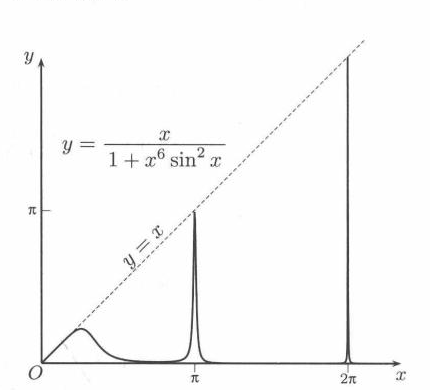
\includegraphics[width=.52\linewidth]{figures/upper/ch12/fig-12-1.png}

  图 12.1
\end{center}

取 $A_n=n\pi,n\in\NN_+$，则可分解积分为
\[
  \int_0^{n\pi}\frac{x\,\dd x}{1+x^6\sin^2x}
  =\sum_{k=1}^n u_k,\qquad
  u_k=\int_{(k-1)\pi}^{k\pi}\frac{x\,\dd x}{1+x^6\sin^2x}.
\]
对于 $u_k$ 可估计如下（$k\geq2$），其中对于区间 $[0,\frac\pi2]$ 上的 $\sin x$ 应用 Jordan 不等式 $\sin x\geq2x/\pi$（例题 8.5.6）：
\begin{align*}
  u_k
  &\leq k\pi\int_{(k-1)\pi}^{k\pi}\frac{\dd x}{1+(k-1)^6\pi^6\sin^2x}\\
  &=k\pi\int_0^\pi\frac{\dd x}{1+(k-1)^6\pi^6\sin^2x}\\
  &=2k\pi\int_0^{\pi/2}\frac{\dd x}{1+(k-1)^6\pi^6\sin^2x}\\
  &\leq2k\pi\int_0^{\pi/2}\frac{\dd x}{1+4(k-1)^6\pi^4x^2}\\
  &=\frac{k}{\pi(k-1)^3}\int_0^{(k-1)^3\pi^3}\frac{\dd t}{1+t^2}
  \sim\frac1{2k^2}\qquad(k\to\infty).
\end{align*}
由于
\[
  1+\frac1{2^2}+\cdots+\frac1{n^2}
  <1+\frac1{1\cdot2}+\cdots+\frac1{(n-1)n}<2
\]
与 $n$ 无关，可见函数值序列 $\{F(n\pi)\}$ 有界，从而函数 $F(A)$ 在 $0\leq A<+\infty$ 上有界，因此本题的广义积分收敛。
\end{xsolution}

\begin{xremark}
如图 12.1 所示，这个收敛积分的被积函数满足等式 $f(k\pi)=k\pi$。这表明函数图像与第一象限的角平分线 $y=x$ 有无穷多个交点。交点的坐标是 $(k\pi,k\pi)$，$k$ 取所有非负整数。但是当 $x\neq k\pi$ 时函数值 $f(x)$ 就急剧下降，当 $x>\pi$ 时函数图像在图 12.1 上已经与 $x$ 轴很难区分开。由这个例子可见，无穷限广义积分 $\int_a^{+\infty}f(x)\,\dd x$ 收敛时，其被积函数的极限 $f(+\infty)$ 不仅可以不存在，而且可以有
\[
  \limsup_{x\to+\infty}f(x)=+\infty
\]
（这里的上极限是 §3.6 中的相应概念在连续情况的推广）。
\end{xremark}

\subsection{练习题}

\begin{xexercise}[1]
讨论下列广义积分的敛散性，若是收敛，还要讨论是条件收敛还是绝对收敛：
  \begin{enumerate}[label=(\arabic*)]
    \item $\displaystyle\int_0^{+\infty}x\sin^4x\,\dd x$；
    \item $\displaystyle\int_3^{+\infty}\frac{\ln\ln x}{\ln x}\sin x\,\dd x$；
    \item $\displaystyle\int_0^{+\infty}\frac1x\ee^{\cos x}\sin(\sin x)\,\dd x$；
    \item $\displaystyle\int_1^{+\infty}\ln\frac{x^2}{x^2-1}\,\dd x$；
    \item $\displaystyle\int_1^{+\infty}\ln\left(\cos\frac1x+\sin\frac1x\right)\,\dd x$；
    \item $\displaystyle\int_0^1\frac1x\ln\frac{1+x}{1-x}\,\dd x$；
    \item $\displaystyle\int_0^{+\infty}\left[\frac1{\sqrt{x}}-\sqrt{\ln\left(1+\frac1x\right)}\right]\,\dd x$；
    \item $\displaystyle\int_0^{+\infty}\frac{\sin x}{\sqrt{x+\cos x}}\,\dd x$。
  \end{enumerate}
\end{xexercise}
\begin{xsolution}
\textbf{(1)} 被积函数非负。取区间
\[
  I_k=\left[k\pi+\frac\pi4,k\pi+\frac{3\pi}4\right],\qquad k\in\NN,
\]
则 $\sin^4x\geq1/4$，从而
\[
  \int_{I_k}x\sin^4x\,\dd x\geq\frac14\cdot\frac\pi2\left(k\pi+\frac\pi4\right).
\]
右边之和发散，故原积分发散。

\textbf{(2)} 令
\[
  a(x)=\frac{\ln\ln x}{\ln x}.
\]
当 $x>\ee^{\ee}$ 时 $a(x)>0$、单调减少且趋于 $0$，而 $\int_3^A\sin x\,\dd x$ 有界，故由 Dirichlet 判别法原积分收敛。另一方面，在每个 $[k\pi,(k+1)\pi]$ 上，$a$ 变化缓慢且 $\int|\sin x|\,\dd x=2$；特别地对充分大的 $k$ 有
\[
  \int_{k\pi}^{(k+1)\pi}a(x)|\sin x|\,\dd x
  \geq 2a((k+1)\pi).
\]
而 $a((k+1)\pi)>1/(k+1)$ 对充分大的 $k$ 成立，因此绝对值积分发散。故为条件收敛。

\textbf{(3)} 记
\[
  h(x)=\ee^{\cos x}\sin(\sin x).
\]
$h$ 是连续的 $2\pi$ 周期函数，且 $h(2\pi-x)=-h(x)$，所以一周期积分为 $0$，其原函数 $\int_0^x h(t)\,\dd t$ 有界。又 $1/x$ 单调趋于 $0$，故无穷远处由 Dirichlet 判别法收敛；在 $0$ 点，$h(x)/x\to\ee$，故无瑕点。因此原积分收敛。由于 $h\not\equiv0$，$|h|$ 的周期平均值严格为正，所以
\[
  \int_1^{+\infty}\frac{|h(x)|}{x}\,\dd x=+\infty.
\]
故原积分条件收敛。

\textbf{(4)} 当 $x\to1+$ 时
\[
  \ln\frac{x^2}{x^2-1}=-\ln(x-1)+\bigO(1),
\]
可积；当 $x\to+\infty$ 时
\[
  \ln\frac{x^2}{x^2-1}=-\ln\left(1-\frac1{x^2}\right)
  \sim\frac1{x^2}.
\]
被积函数为正，故积分绝对收敛。进一步，
\[
  \int \ln\frac{x^2}{x^2-1}\,\dd x
  =x\ln\frac{x^2}{x^2-1}+\ln(x-1)-\ln(x+1)+C,
\]
而右边无常数项部分在 $x\to+\infty$ 时趋于 $0$，在 $x\to1+$ 时趋于 $-\ln4$，所以
\[
  \int_1^{+\infty}\ln\frac{x^2}{x^2-1}\,\dd x=\boxed{\ln4}.
\]

\textbf{(5)} 当 $x\to+\infty$ 时，令 $u=1/x$，则
\[
  \ln(\cos u+\sin u)=u+\bigO(u^2),
\]
所以被积函数与 $1/x$ 等价，原积分发散到 $+\infty$。

\textbf{(6)} 当 $x\to0+$ 时
\[
  \frac1x\ln\frac{1+x}{1-x}=2+\bigO(x^2),
\]
当 $x\to1-$ 时
\[
  \frac1x\ln\frac{1+x}{1-x}=-\ln(1-x)+\bigO(1).
\]
两端都可积，且被积函数非负，故绝对收敛。

\textbf{(7)} 因 $\ln(1+u)<u$（$u>0$），被积函数为正。当 $x\to0+$ 时，两项分别为 $x^{-1/2}$ 与 $\bigO(\sqrt{|\ln x|})$，均可积；当 $x\to+\infty$ 时
\[
  \sqrt{\ln\left(1+\frac1x\right)}
  =\frac1{\sqrt x}\left(1-\frac1{4x}+\bigO(x^{-2})\right),
\]
故差为
\[
  \frac1{4x^{3/2}}+\bigO(x^{-5/2}).
\]
因此原积分绝对收敛。

\textbf{(8)} 令
\[
  a(x)=\frac1{\sqrt{x+\cos x}}.
\]
因为 $x+\cos x$ 单调不减且大于 $0$，故 $a(x)$ 单调不增并趋于 $0$。由 Dirichlet 判别法原积分收敛。又 $a(x)\sim x^{-1/2}$，故
\[
  \int_1^{+\infty}|\sin x|a(x)\,\dd x
\]
与 $\int_1^{+\infty}|\sin x|x^{-1/2}\,\dd x$ 同敛散，后者发散，因此原积分条件收敛。
\end{xsolution}


\begin{xexercise}[2]
对于以下含有参数的广义积分，确定出使积分绝对收敛、条件收敛和发散的参数范围：
  \begin{enumerate}[label=(\arabic*)]
    \item $\displaystyle\int_0^{\pi/2}\frac{\dd x}{\sin^p x\cos^q x}$；
    \item $\displaystyle\int_0^{+\infty}\frac{\cos x}{1+x^p}\,\dd x\quad(p>0)$；
    \item $\displaystyle\int_0^{+\infty}\frac{\sin x}{x}\abs{\ln x}^p\,\dd x$；
    \item $\displaystyle\int_0^{+\infty}\frac{\ln(1+x)}{x^p}\,\dd x$；
    \item $\displaystyle\int_0^{+\infty}\frac{\sin x^2}{1+x^p}\,\dd x\quad(p\geq0)$；
    \item $\displaystyle\int_0^{+\infty}\frac{x^p\sin x}{1+x^q}\,\dd x$；
    \item $\displaystyle\int_0^{+\infty}\frac{\ee^{\sin x}\sin2x}{x^p}\,\dd x$；
    \item $\displaystyle\int_{\ee}^{+\infty}\frac{\dd x}{(x-\ee)^p(\ln\ln x)^q}$。
  \end{enumerate}
\end{xexercise}
\begin{xsolution}
\textbf{(1)} 在 $0$ 附近被积函数与 $x^{-p}$ 等价，在 $\pi/2$ 附近与 $(\pi/2-x)^{-q}$ 等价。因此
\[
  \boxed{p<1,\ q<1}
\]
时绝对收敛；否则发散。因被积函数非负，无条件收敛情形。

\textbf{(2)} 对 $p>0$，无穷远处由 Dirichlet 判别法总收敛；绝对收敛当且仅当 $p>1$。所以
\[
  \boxed{p>1\text{ 时绝对收敛； }0<p\leq1\text{ 时条件收敛}.}
\]

\textbf{(3)} 在 $x=0$ 邻近，$\sin x/x\to1$，且对任意实数 $p$，作 $t=-\ln x$ 可知
\[
  \int_0^{1/2}|\ln x|^p\,\dd x
  =\int_{\ln2}^{+\infty}t^p\ee^{-t}\,\dd t<+\infty,
\]
所以 $x=0$ 不产生额外限制。在 $x=1$ 邻近，$|\ln x|^p\sim|x-1|^p$，故局部可积当且仅当 $p>-1$。

当 $x\to+\infty$ 时，$(\ln x)^p/x\to0$ 且最终单调减少，因此在 $p>-1$ 时尾积分由 Dirichlet 判别法收敛。另一方面，绝对值积分在无穷远处与
$\int (\ln x)^p\,\dd x/x$ 同敛散，后者仅在 $p<-1$ 时收敛，这与 $x=1$ 处的局部条件不相容。故
\[
  \boxed{p>-1\text{ 时条件收敛； }p\leq-1\text{ 时发散}.}
\]

\textbf{(4)} 当 $x\to0+$ 时被积函数与 $x^{1-p}$ 等价，需 $p<2$；当 $x\to+\infty$ 时与 $(\ln x)x^{-p}$ 同阶，需 $p>1$。故
\[
  \boxed{1<p<2\text{ 时绝对收敛；其余 }p\text{ 发散}.}
\]

\textbf{(5)} 在 $0$ 点无问题。令 $t=x^2$，绝对值积分在无穷远处等价于
\[
  \frac12\int^{+\infty}\frac{|\sin t|}{t^{(p+1)/2}}\,\dd t,
\]
故绝对收敛当且仅当 $p>1$。而不取绝对值时，$p=0$ 已是 Fresnel 型积分，$p>0$ 更由分部积分或 Dirichlet 判别得到收敛。因此
\[
  \boxed{p>1\text{ 时绝对收敛； }0\leq p\leq1\text{ 时条件收敛}.}
\]

\textbf{(6)} 设
\[
  I=\int_0^{+\infty}\frac{x^p\sin x}{1+x^q}\,\dd x.
\]
若 $q>0$，则 $x\to0+$ 时被积函数与 $x^{p+1}$ 同阶，要求 $p>-2$；无穷远处振幅与 $x^{p-q}$ 同阶，所以收敛要求 $p<q$，绝对收敛要求 $p<q-1$。因而
\[
  \boxed{q>0:\quad
  \begin{cases}
  \text{绝对收敛},&-2<p<q-1,\\
  \text{条件收敛},&p>-2,\ q-1\leq p<q,\\
  \text{发散},&\text{其余情形}.
  \end{cases}}
\]
若 $q=0$，则两端条件分别为 $p>-2$ 与 $p<0$，绝对收敛还需 $p<-1$，故
\[
  \boxed{q=0:\ -2<p<-1\text{ 绝对收敛； }-1\leq p<0\text{ 条件收敛；其余发散}.}
\]
若 $q<0$，则 $x\to0+$ 时被积函数与 $x^{p-q+1}$ 同阶，要求 $p>q-2$；无穷远处与 $x^p\sin x$ 同型。因此
\[
  \boxed{q<0:\quad
  \begin{cases}
  \text{绝对收敛},&q-2<p<-1,\\
  \text{条件收敛},&-1\leq p<0,\\
  \text{发散},&p\leq q-2\text{ 或 }p\geq0.
  \end{cases}}
\]

\textbf{(7)} 记 $h(x)=\ee^{\sin x}\sin2x$。它为 $2\pi$ 周期函数，且
\[
  h(x)=\frac{\dd}{\dd x}\bigl(2(\sin x-1)\ee^{\sin x}\bigr),
\]
故一周期积分为 $0$，原函数有界。无穷远处因此在 $p>0$ 时由 Dirichlet 判别法收敛；绝对收敛当且仅当 $p>1$。在 $0$ 点有 $h(x)\sim2x$，故局部条件为 $p<2$。综上
\[
  \boxed{1<p<2\text{ 时绝对收敛； }0<p\leq1\text{ 时条件收敛； }p\leq0\text{ 或 }p\geq2\text{ 时发散}.}
\]

\textbf{(8)} 当 $x\to\ee+$ 时
\[
  \ln\ln x\sim\frac{x-\ee}{\ee},
\]
故局部可积当且仅当 $p+q<1$。当 $x\to+\infty$ 时，被积函数与
\[
  \frac1{x^p(\ln\ln x)^q}
\]
同阶；该正函数的积分收敛当且仅当 $p>1$（$p=1$ 时令 $t=\ln x$，得到 $\int\dd t/(\ln t)^q$，对任意 $q$ 都发散）。因此
\[
  \boxed{p>1,\quad p+q<1}
\]
时绝对收敛，其余情形发散；无条件收敛情形。
\end{xsolution}


\begin{xexercise}[3]
设 $a_1,\ldots,a_n$ 为互不相同的实数，$p_1,\ldots,p_n>0$，讨论广义积分
  \[
    \int_{-\infty}^{+\infty}\frac{\dd x}{\abs{x-a_1}^{p_1}\abs{x-a_2}^{p_2}\cdots\abs{x-a_n}^{p_n}}
  \]
  的敛散性。
\end{xexercise}
\begin{xsolution}
在每个有限奇点 $a_i$ 邻近，被积函数与 $C_i|x-a_i|^{-p_i}$ 等价，所以必须且只需
\[
  p_i<1\qquad(i=1,\ldots,n).
\]
当 $|x|\to\infty$ 时，被积函数与 $|x|^{-P}$ 等价，其中 $P=p_1+\cdots+p_n$，故无穷远处可积当且仅当 $P>1$。因此
\[
  \boxed{p_i<1\ (1\leq i\leq n),\qquad \sum_{i=1}^n p_i>1}
\]
是收敛的充分必要条件。
\end{xsolution}


\begin{xexercise}[4]
讨论广义积分
  \[
    \int_0^{+\infty}\left[\ln\left(1+\frac1x\right)-\frac1{1+x}\right]\,\dd x
  \]
  的敛散性。
\end{xexercise}
\begin{xsolution}
被积函数为正。$x\to0+$ 时
\[
  \ln\left(1+\frac1x\right)-\frac1{1+x}
  =\ln\frac1x+\bigO(1),
\]
可积；$x\to+\infty$ 时
\[
  \ln\left(1+\frac1x\right)-\frac1{1+x}
  =\frac1{2x^2}+\bigO(x^{-3}).
\]
所以原积分绝对收敛。又因为
\[
  \frac{\dd}{\dd x}\left[x\ln\left(1+\frac1x\right)\right]
  =\ln\left(1+\frac1x\right)-\frac1{1+x},
\]
且
\[
  \lim_{x\to0+}x\ln\left(1+\frac1x\right)=0,
  \qquad
  \lim_{x\to+\infty}x\ln\left(1+\frac1x\right)=1,
\]
故还可得到
\[
  \int_0^{+\infty}\left[\ln\left(1+\frac1x\right)-\frac1{1+x}\right]\,\dd x=\boxed{1}.
\]
\end{xsolution}


\begin{xexercise}[5]
判别广义积分
  \[
    \int_0^{+\infty}\frac{x\,\dd x}{1+x^4\sin^2x}
  \]
  的敛散性。
\end{xexercise}
\begin{xsolution}
令
\[
  F(A)=\int_0^A\frac{x\,\dd x}{1+x^4\sin^2x}.
\]
被积函数为正。对充分大的整数 $k$，在
\[
  J_k=\left[k\pi-\frac1{(k\pi)^2},\ k\pi+\frac1{(k\pi)^2}\right]
\]
上有 $x\geq k\pi/2$，且 $|\sin x|\leq|x-k\pi|$。于是
\[
  x^4\sin^2x\leq (2k\pi)^4\frac1{(k\pi)^4}=16,
\]
从而
\[
  \int_{J_k}\frac{x\,\dd x}{1+x^4\sin^2x}
  \geq \frac{k\pi/2}{17}\cdot\frac{2}{(k\pi)^2}
  =\frac1{17k\pi}.
\]
这些区间最终互不相交，右边为调和级数型，故原积分发散。
\end{xsolution}


\begin{xexercise}[6]
求函数
  \[
    F(x)=\int_0^{+\infty}\abs*{t^2-\frac1{t^2}}^x\,\dd t
  \]
  的定义域。
\end{xexercise}
\begin{xsolution}
当 $t\to0+$ 时
\[
  \left|t^2-\frac1{t^2}\right|^x\sim t^{-2x},
\]
故需 $x<1/2$；当 $t\to+\infty$ 时与 $t^{2x}$ 等价，故需 $x<-1/2$；当 $t\to1$ 时
\[
  \left|t^2-\frac1{t^2}\right|^x\sim4^x|t-1|^x,
\]
故需 $x>-1$。三者合并得定义域
\[
  \boxed{(-1,-1/2)}.
\]
\end{xsolution}


\begin{xexercise}[7]
设 $f'\in C[0,1]$ 且 $f'(x)$ 处处大于 0，证明：广义积分
  \[
    \int_0^1\frac{f(x)-f(0)}{x^p}\,\dd x
  \]
  在 $p<2$ 时收敛，$p\geq2$ 时发散。
\end{xexercise}
\begin{xsolution}
由 $f'\in C[0,1]$ 且 $f'(0)>0$，Taylor 公式给出
\[
  f(x)-f(0)=f'(0)x+\littleo(x)\qquad(x\to0+).
\]
所以被积函数与 $f'(0)x^{1-p}$ 等价。于是 $1-p>-1$，即 $p<2$ 时收敛；$p\geq2$ 时发散。由于 $f'(x)>0$，被积函数在 $(0,1]$ 上为正，故发散时确为趋于 $+\infty$。
\end{xsolution}


\begin{xexercise}[8]
设 $\int_a^{+\infty}f$ 为条件收敛，证明：
  \begin{enumerate}[label=(\arabic*)]
    \item 广义积分 $\int_a^{+\infty}(\abs{f}\pm f)$ 发散；
    \item $\displaystyle\lim_{x\to+\infty}\frac{\int_a^x(\abs{f}+f)}{\int_a^x(\abs{f}-f)}=1$。
  \end{enumerate}
\end{xexercise}
\begin{xsolution}
令
\[
  P(x)=\frac{|f(x)|+f(x)}2,\qquad N(x)=\frac{|f(x)|-f(x)}2.
\]
则 $P,N\geq0$，$f=P-N$，$|f|=P+N$。由于 $\int_a^{+\infty}f$ 收敛而 $\int_a^{+\infty}|f|$ 发散，必有
\[
  \int_a^xP\to+\infty,\qquad \int_a^xN\to+\infty,
\]
且
\[
  \int_a^xP-\int_a^xN=\int_a^x f
\]
有有限极限。

\textbf{(1)} 因 $|f|+f=2P$，$|f|-f=2N$，两积分均发散。

\textbf{(2)} 记 $P_x=\int_a^xP$，$N_x=\int_a^xN$。则 $P_x-N_x=\bigO(1)$，而 $N_x\to+\infty$，故
\[
  \frac{\int_a^x(|f|+f)}{\int_a^x(|f|-f)}
  =\frac{P_x}{N_x}=1+\frac{P_x-N_x}{N_x}\to1.
\]
\end{xsolution}


\begin{xexercise}[9]
设 $f\in C^1[a,+\infty)$ 单调，且 $f(+\infty)=0$，证明：$\int_a^{+\infty}f'(x)\sin^2x\,\dd x$ 收敛。
\end{xexercise}
\begin{xsolution}
$f$ 单调且 $f(+\infty)=0$。若 $f$ 单调减少，则 $f'\leq0$ 且
\[
  \int_a^{+\infty}|f'(x)|\,\dd x
  =f(a)-f(+\infty)=f(a)<+\infty;
\]
单调增加时同理。因此
\[
  \int_a^{+\infty}|f'(x)\sin^2x|\,\dd x
  \leq\int_a^{+\infty}|f'(x)|\,\dd x<+\infty,
\]
故所给积分绝对收敛。
\end{xsolution}


\begin{xexercise}[10]
设 $f,g\in C^1[a,+\infty)$，$f'(x)$ 非负，$f(+\infty)=0$，且 $g(x)$ 在 $[a,+\infty)$ 上有界，证明：$\int_a^{+\infty}f(x)g'(x)\,\dd x$ 收敛。
\end{xexercise}
\begin{xsolution}
由 $f'\geq0$ 且 $f(+\infty)=0$，知 $f(x)\leq0$，且
\[
  \int_a^{+\infty}f'(x)\,\dd x=-f(a)<+\infty.
\]
设 $|g(x)|\leq M$。在 $[a,A]$ 上分部积分：
\[
  \int_a^A f(x)g'(x)\,\dd x
  =f(A)g(A)-f(a)g(a)-\int_a^A f'(x)g(x)\,\dd x.
\]
第一项因 $f(A)\to0$ 且 $g$ 有界而趋于 $0$，最后一项绝对收敛，因为
\[
  \int_a^{+\infty}|f'(x)g(x)|\,\dd x\leq M\int_a^{+\infty}f'(x)\,\dd x<+\infty.
\]
故原广义积分收敛。
\end{xsolution}


\section{广义积分的计算}

广义积分是定积分与函数极限的结合，因此定积分计算的公式与技巧几乎都能应用于广义积分。这方面的例题放在下面第一小节中。第二小节则专门介绍几个特殊广义积分的计算，它们都有重要的应用，也都需要用特殊的技巧来计算。

与常义积分的计算不同之处是，在计算一个广义积分之前应当先观察它是否收敛，如果该广义积分是发散的，就不必做无用功了。（在某些问题中这时还需要考虑其主值是否存在和怎样计算的问题。）

\subsection{例题}

\begin{xexample}[12.3.1]
计算广义积分
\[
  I=\int_0^{+\infty}\frac{\ln x}{1+x^2}\,\dd x.
\]
\end{xexample}
\begin{xsolution}
这时的积分以 0 和 $+\infty$ 为奇点，容易验证其收敛性。因此可以将积分拆开成两个积分：
\[
  \int_0^{+\infty}\frac{\ln x}{1+x^2}\,\dd x
  =\int_0^1\frac{\ln x}{1+x^2}\,\dd x
  +\int_1^{+\infty}\frac{\ln x}{1+x^2}\,\dd x,
\]
然后对上式右边的第二个积分作倒代换，就得到
\[
  \int_1^{+\infty}\frac{\ln x}{1+x^2}\,\dd x
  =-\int_0^1\frac{\ln x}{1+x^2}\,\dd x,
\]
因此原广义积分等于 0。
\end{xsolution}

\begin{xremark}
以上计算的实质是什么？试作代换 $x=\tan t$，就得到
\[
  I=\int_0^{\pi/2}\ln\tan t\,\dd t.
\]
由于
\[
  \ln\tan\left(\frac\pi2-t\right)=\ln\cot t=-\ln\tan t,
\]
因此被积函数 $\ln\tan t$ 在区间 $(0,\pi/2)$ 上关于区间中点为奇函数。如果与命题 10.4.5 作比较，可见积分等于 0 的原因在于对称性。关于命题 10.4.5 在广义积分情况下的推广留作为 12.3.3 小节的练习题 1。
\end{xremark}

\begin{xexample}[12.3.2]
计算广义积分
\[
  \int_0^1(\ln x)^n\,\dd x,\qquad n\in\NN_+.
\]
\end{xexample}
\begin{xsolution}
这是一个无界积分，$x=0$ 是瑕点。由 $\lim_{x\to0+}x^{1/2}(\ln x)^n=0$，知所求广义积分收敛。设 $I_n=\int_0^1(\ln x)^n\,\dd x$，应用分部积分法得到
\begin{align*}
  I_n
  &=x(\ln x)^n\big|_{0+}^1-\int_0^1n(\ln x)^{n-1}\,\dd x
  =-n\int_0^1(\ln x)^{n-1}\,\dd x=-nI_{n-1}\\
  &=(-1)^2n(n-1)I_{n-2}=\cdots=(-1)^nn!I_0=(-1)^nn!.
\end{align*}
\end{xsolution}

在广义积分计算中也可以用分部积分，但这时需要注意，如果在积分外出现非有限数，则不能得到正确结果。

\begin{xexample}[12.3.3]
计算广义积分
\[
  \int_0^{+\infty}\frac{x\ln x}{(1+x^2)^2}\,\dd x.
\]
\end{xexample}

\textbf{分析}\quad 这个广义积分的收敛性是容易判别的，而且 $x=0$ 不是瑕点。为了计算它的值，可以用与例题 12.3.1 完全相同的方法，答案也是 0，同时那里的注解对本题也一样有效，细节从略。

但是由于本题的被积函数的形式，容易使我们产生用分部积分的想法。这时用分部积分得到
\begin{align*}
  \int_0^{+\infty}\frac{x\ln x}{(1+x^2)^2}\,\dd x
  &=\int_0^{+\infty}\ln x\,\dd\left(-\frac1{2(1+x^2)}\right)\\
  &=-\frac{\ln x}{2(1+x^2)}\bigg|_{0+}^{+\infty}
  +\int_0^{+\infty}\frac{\dd x}{2x(1+x^2)}.
\end{align*}
这时右边的第一项当 $x\to0+$ 时发散，同时最后一个积分也发散，出现了 $\infty-\infty$ 型的不定式。造成错误的原因是忽视了运用广义积分分部积分法的基本条件：在 $\int_a^b u\,\dd v$，$\int_a^b v\,\dd u$，$uv\big|_a^b$ 中至少要知道已有两个收敛。

\begin{xremark}
类似的问题对于常义积分也是存在的，这在例题 10.4.1 中已经遇到过，但对于广义积分却难以用那里介绍的待定常数法来解决。当然，也可以如例题 9.1.5 那样，用分部积分法先求出本题的被积函数的不定积分，然后用广义的 Newton-Leibniz 公式进行计算。
\end{xremark}

\subsection{几个特殊广义积分的计算}

本节介绍几个有名的广义积分，其中的方法和结果都是重要的。利用这些积分还可以计算出很多其他积分（见下一小节的练习题 3--6）。

\begin{xexample}[12.3.4（Euler 积分）]
计算积分
\[
  I=\int_0^{\pi/2}\ln\sin x\,\dd x.
\]
\end{xexample}
\begin{xsolution}
\textbf{解 1}\quad 这是无界积分，瑕点为 $x=0$。利用 Cauchy 判别法，容易验证其收敛性。应用命题 10.4.6 在无界积分情况下的推广就容易计算如下：
\begin{align*}
  I
  &=\int_0^{\pi/4}(\ln\sin x+\ln\cos x)\,\dd x
   =\int_0^{\pi/4}(\ln\sin2x-\ln2)\,\dd x\\
  &=\frac12\int_0^{\pi/2}\ln\sin y\,\dd y-\frac\pi4\ln2
   =\frac12I-\frac\pi4\ln2,
\end{align*}
所以 $I=-\dfrac\pi2\ln2$。

\textbf{解 2}\quad 先作代换 $x=2t$，得到
\[
  I=\int_0^{\pi/4}2\ln\sin2t\,\dd t
   =\frac\pi2\ln2+\int_0^{\pi/4}2\ln\sin t\,\dd t
   +\int_0^{\pi/4}2\ln\cos t\,\dd t,
\]
对右边最后一个积分用代换 $t=\pi/2-u$，得到
\begin{align*}
  I
  &=\frac\pi2\ln2+\int_0^{\pi/4}2\ln\sin t\,\dd t
   +\int_{\pi/4}^{\pi/2}2\ln\sin u\,\dd u\\
  &=\frac\pi2\ln2+\int_0^{\pi/2}2\ln\sin t\,\dd t
   =\frac\pi2\ln2+2I,
\end{align*}
所以 $I=-\dfrac\pi2\ln2$。
\end{xsolution}

\begin{xexample}[12.3.5（Froullani（伏龙兰尼）积分）]
设函数 $f$ 在 $[0,+\infty)$ 上连续，极限 $f(+\infty)$ 存在且有限，$0<a<b$，计算积分
\[
  \int_0^{+\infty}\frac{f(ax)-f(bx)}x\,\dd x.
\]
\end{xexample}
\begin{xsolution}
本题的广义积分的收敛性将在下面的计算过程中建立。对 $0<r<R<+\infty$，由定积分的换元积分法，成立
\begin{align*}
  \int_r^R\frac{f(ax)-f(bx)}x\,\dd x
  &=\int_r^R\frac{f(ax)}x\,\dd x-\int_r^R\frac{f(bx)}x\,\dd x\\
  &=\int_{ar}^{aR}\frac{f(x)}x\,\dd x-\int_{br}^{bR}\frac{f(x)}x\,\dd x\\
  &=\int_{ar}^{br}\frac{f(x)}x\,\dd x-\int_{aR}^{bR}\frac{f(x)}x\,\dd x.
\end{align*}
对上式右边的两个定积分分别应用积分第一中值定理，得到
\[
  \int_{ar}^{br}\frac{f(x)}x\,\dd x
  =f(\xi)\int_{ar}^{br}\frac{\dd x}x
  =f(\xi)\ln\frac ba\qquad(ar<\xi<br),
\]
\[
  \int_{aR}^{bR}\frac{f(x)}x\,\dd x
  =f(\eta)\int_{aR}^{bR}\frac{\dd x}x
  =f(\eta)\ln\frac ba\qquad(aR<\eta<bR).
\]
在上两式中分别令 $r\to0+$，$R\to+\infty$，注意到这时 $\xi\to0+$，$\eta\to+\infty$，由于 $f(0+)=f(0)$，$f(+\infty)$ 存在且有限，而且 $\int_r^R\frac{f(ax)-f(bx)}x\,\dd x$ 在这时的极限就是 Froullani 积分，便得到
\[
  \int_0^{+\infty}\frac{f(ax)-f(bx)}x\,\dd x
  =[f(0)-f(+\infty)]\ln\frac ba.
\]
\end{xsolution}

\begin{xremark}
从上面的证明过程可以得到 Froullani 积分的两种变形：
\begin{enumerate}[label=(\arabic*)]
  \item 若 $x\to+\infty$ 时 $f(x)$ 没有有限极限，但是对某个 $A>0$，积分 $\int_A^{+\infty}\frac{f(x)}x\,\dd x$ 收敛，则有
  \[
    \int_0^{+\infty}\frac{f(ax)-f(bx)}x\,\dd x=f(0)\ln\frac ba.
  \]
  \item 若 $f$ 在 0 点不连续，甚至右极限也不存在，但对于某个 $A>0$，积分 $\int_0^A\frac{f(x)}x\,\dd x$ 收敛，则有
  \[
    \int_0^{+\infty}\frac{f(ax)-f(bx)}x\,\dd x=f(+\infty)\ln\frac ba.
  \]
\end{enumerate}
\end{xremark}

\begin{xexample}[12.3.6（Dirichlet 积分）]
证明：积分
\[
  \int_0^{+\infty}\frac{\sin x}{x}\,\dd x=\frac\pi2.
\]
\end{xexample}
\begin{xsolution}
从例题 12.2.3 已知这个广义积分为条件收敛。为了计算它的值，要利用在例题 10.4.3 中已经得到的结果（也有称为 Dirichlet 积分的）：
\[
  \int_0^\pi\frac{\sin\left(n+\frac12\right)x}{2\sin\frac x2}\,\dd x=\frac\pi2.
\]
先观察将其分母换为 $x$ 所产生的影响。用 L'Hospital 法则，有
\[
  f(x)=\frac1x-\frac1{2\sin\frac x2}=\bigO(x)\qquad(x\to0),
\]
因此 $f$ 在 $[0,\pi]$ 上常义可积。应用 Riemann 引理（例题 10.2.6），有
\[
  \lim_{n\to\infty}\int_0^\pi f(x)\sin\left(n+\frac12\right)x\,\dd x=0,
\]
并且得到
\[
  \lim_{n\to\infty}\int_0^\pi\frac{\sin\left(n+\frac12\right)x}{x}\,\dd x
  =\lim_{n\to\infty}\int_0^\pi\frac{\sin\left(n+\frac12\right)x}{2\sin\frac x2}\,\dd x=\frac\pi2.
\]
最后在利用代换得到的等式
\[
  \int_0^\pi\frac{\sin\left(n+\frac12\right)x}{x}\,\dd x
  =\int_0^{(n+\frac12)\pi}\frac{\sin t}{t}\,\dd t
\]
的两边令 $n\to\infty$，就得到所要的结果。
\end{xsolution}

下面的一个广义积分称为概率积分（也称为 Euler-Poisson 积分），它的值在概率统计中是一个基本量。

\begin{xexample}[12.3.7（Euler-Poisson 积分）]
证明：积分
\[
  \int_0^{+\infty}\ee^{-t^2}\,\dd t=\frac{\sqrt\pi}{2}.
\]
\end{xexample}
\begin{xsolution}
积分的收敛性是明显的。利用对于每个 $t$，数列 $\{(1-t^2/n)^n\}$ 的极限是 $\ee^{-t^2}$，我们研究积分
\[
  I_n=\int_0^{\sqrt n}\left(1-\frac{t^2}n\right)^n\,\dd t.
\]
作代换 $t=\sqrt n\sin x$，就有
\[
  I_n=\sqrt n\int_0^{\pi/2}\cos^{2n+1}x\,\dd x
  =\sqrt n\cdot\frac{(2n)!!}{(2n+1)!!}\to\frac{\sqrt\pi}{2}\qquad(n\to\infty).
\]
这里利用了例题 10.4.9 和 Wallis 公式 (11.29)。由于右边的极限值已经是概率积分的数值，而且又有
\[
  \int_0^{+\infty}\ee^{-t^2}\,\dd t
  =\lim_{n\to\infty}\int_0^{\sqrt n}\ee^{-t^2}\,\dd t,
\]
因此只需要再证明
\[
  \lim_{n\to\infty}\int_0^{\sqrt n}\left[\ee^{-t^2}-\left(1-\frac{t^2}n\right)^n\right]\,\dd t=0.
\]
利用关于指数函数的一个不等式（见例题 8.5.4）：当 $a\geq1$ 时在区间 $[0,a]$ 上成立
\begin{equation}
  0\leq\ee^{-x}-\left(1-\frac xa\right)^a\leq\frac{x^2}{a}\ee^{-x},
  \tag{12.7}
  \label{eq:12.7}
\end{equation}
在其中令 $x=t^2,a=n$，就得到估计式
\[
  0\leq\int_0^{\sqrt n}\left[\ee^{-t^2}-\left(1-\frac{t^2}n\right)^n\right]\,\dd t
  \leq\frac{\int_0^{\sqrt n}t^4\ee^{-t^2}\,\dd t}{n}.
\]
由于当 $n\to\infty$ 时右边分子上的广义积分收敛，因此右边极限为 0。
\end{xsolution}

\begin{xremark}
计算概率积分的方法很多，比较传统的方法有：(1) 从简单不等式
\begin{equation}
  1-x^2\leq\ee^{-x^2}\leq\frac1{1+x^2}\qquad(x\geq0)
  \tag{12.8}
  \label{eq:12.8}
\end{equation}
出发，用夹逼方法，见 [14] 第二卷 492 小节（留作为第二组参考题 1）；(2) 二重广义积分方法，见 [14] 第三卷 617 小节与本书下册例题 22.4.1；(3) 含参积分中交换积分次序的方法，见 [14] 第二卷 522 小节；(4) 对广义积分取极限的方法，见本书下册例题 16.1.2。上面所用的方法见《美国数学月刊》(1956) 第 63 卷 35--37 页。
\end{xremark}

\subsection{练习题}

\begin{xexercise}[1]
根据例题 12.3.1 的注，
  \begin{enumerate}[label=(\arabic*)]
    \item 写出命题 10.4.5 在广义积分情况下的推广，并作出证明；
    \item 推广该例题，也就是说当 $f$ 在区间 $[0,+\infty)$ 上满足什么条件时，可以利用类似的方法，或命题 10.4.5 的推广形式，证明 $f$ 在这个区间上的广义积分等于 0。
  \end{enumerate}
\end{xexercise}
\begin{xsolution}
\textbf{(1)} 广义积分情形的对称性命题可表述为：设 $f$ 在 $(a,b)$ 上内闭可积，端点或内部允许有瑕点，并假定 $\int_a^b f(x)\,\dd x$ 收敛。若
\[
  f(a+b-x)=-f(x)\qquad(a<x<b),
\]
则
\[
  \int_a^b f(x)\,\dd x=0.
\]
证明如下。对避开所有瑕点的截断积分作代换 $x=a+b-t$，得到
\[
  \int f(x)\,\dd x=-\int f(t)\,\dd t
\]
（上下限同时按对称方式截断）。由于原广义积分收敛，可以让各截断端点趋于相应奇点并分别取极限，于是积分值等于其相反数，只能为 $0$。若奇点位于区间中点，则应先按广义积分定义在该点左右分别判定收敛，再作上述代换，不能仅用主值代替。

\textbf{(2)} 对 $[0,+\infty)$，例题 12.3.1 所用倒代换给出一个方便的推广：若 $f$ 在 $(0,+\infty)$ 上内闭可积，$\int_0^1f$ 与 $\int_1^{+\infty}f$ 都收敛，并且
\[
  f(1/x)=-x^2f(x)\qquad(x>0),
\]
则
\begin{align*}
  \int_1^{+\infty}f(x)\,\dd x
  &=\int_0^1\frac{f(1/t)}{t^2}\,\dd t
  =-\int_0^1f(t)\,\dd t,
\end{align*}
从而 $\int_0^{+\infty}f=0$。等价地，作 $x=\tan t$ 后，只要
\[
  f(\tan(\tfrac\pi2-t))\sec^2(\tfrac\pi2-t)
  =-f(\tan t)\sec^2t,
\]
且相应广义积分收敛，也可由关于 $\pi/4$ 的反对称性得到积分为 $0$。
\end{xsolution}


\begin{xexercise}[2]
计算下列广义积分：
  \begin{enumerate}[label=(\arabic*)]
    \item $\displaystyle\int_0^{+\infty}\ee^{-x}\abs{\sin x}\,\dd x$；
    \item $\displaystyle\int_1^{+\infty}\frac{\dd x}{\ee^{x+1}+\ee^{3-x}}$；
    \item $\displaystyle\int_a^b\frac{\dd x}{\sqrt{(x-a)(b-x)}}$；
    \item $\displaystyle\int_0^{+\infty}\frac{\dd x}{(1+x^2)^n}\quad(n\in\NN_+)$；
    \item $\displaystyle\int_0^1x^n\left(\ln\frac1x\right)^m\,\dd x\quad(n,m\in\NN_+)$；
    \item $\displaystyle\int_0^{+\infty}\frac{\sin\left(x-\frac1x\right)}x\,\dd x$；
    \item $\displaystyle\int_0^{+\infty}\frac{\ln x}{(x^2+1)(x^2+4)}\,\dd x$；
    \item $\displaystyle\int_{-1}^1\frac{\dd}{\dd x}\left(\frac1{1+2^{1/x}}\right)\,\dd x$。
  \end{enumerate}
\end{xexercise}
\begin{xsolution}
\textbf{(1)} 利用 $|\sin x|$ 的周期为 $\pi$，有
\[
  I=\sum_{k=0}^{\infty}\int_{k\pi}^{(k+1)\pi}\ee^{-x}|\sin x|\,\dd x
  =\sum_{k=0}^{\infty}\ee^{-k\pi}\int_0^\pi\ee^{-t}\sin t\,\dd t.
\]
而
\[
  \int_0^\pi\ee^{-t}\sin t\,\dd t=\frac{1+\ee^{-\pi}}2.
\]
故
\[
  \boxed{I=\frac{1+\ee^{-\pi}}{2(1-\ee^{-\pi})}
  =\frac12\operatorname{coth}\frac\pi2.}
\]

\textbf{(2)} 令 $u=x-1$，则
\[
  \ee^{x+1}+\ee^{3-x}=\ee^2(\ee^u+\ee^{-u}),
\]
所以
\[
  I=\ee^{-2}\int_0^{+\infty}\frac{\dd u}{\ee^u+\ee^{-u}}
  =\frac{\ee^{-2}}2\int_0^{+\infty}\operatorname{sech}u\,\dd u
  =\boxed{\frac\pi{4\ee^2}}.
\]

\textbf{(3)} 作
\[
  x=\frac{a+b}2+\frac{b-a}2\cos t,
\]
则 $\sqrt{(x-a)(b-x)}=(b-a)\sin t/2$，故
\[
  \boxed{\int_a^b\frac{\dd x}{\sqrt{(x-a)(b-x)}}=\pi.}
\]

\textbf{(4)} 令 $x=\tan t$，得
\[
  I_n=\int_0^{\pi/2}\cos^{2n-2}t\,\dd t
  =\boxed{\frac\pi2\frac{(2n-3)!!}{(2n-2)!!}}
  \qquad(n\in\NN_+).
\]

\textbf{(5)} 令 $t=-(n+1)\ln x$，则
\[
  I=\frac1{(n+1)^{m+1}}\int_0^{+\infty}t^m\ee^{-t}\,\dd t
  =\boxed{\frac{m!}{(n+1)^{m+1}}}.
\]

\textbf{(6)} 将积分在 $1$ 处分开。对 $(0,1)$ 作 $x=1/t$，得到
\[
  \int_0^1\frac{\sin(x-1/x)}x\,\dd x
  =-\int_1^{+\infty}\frac{\sin(t-1/t)}t\,\dd t.
\]
两部分都按 Dirichlet 型方法收敛，故
\[
  \boxed{I=0}.
\]

\textbf{(7)} 分式分解为
\[
  \frac1{(x^2+1)(x^2+4)}
  =\frac13\left(\frac1{x^2+1}-\frac1{x^2+4}\right).
\]
又令
\[
  J(a)=\int_0^{+\infty}\frac{\ln x}{x^2+a^2}\,\dd x.
\]
作 $x=at$，并用例题 12.3.1 的 $\int_0^{+\infty}\ln t/(1+t^2)\,\dd t=0$，得
\[
  J(a)=\frac\pi{2a}\ln a.
\]
所以
\[
  \boxed{I=\frac13[J(1)-J(2)]=-\frac\pi{12}\ln2.}
\]

\textbf{(8)} 记
\[
  F(x)=\frac1{1+2^{1/x}}.
\]
则 $F(0-)=1$，$F(0+)=0$，$F(-1)=2/3$，$F(1)=1/3$。按广义积分定义在 $0$ 两侧分别积分，得
\[
  \int_{-1}^1F'(x)\,\dd x
  =[F(0-)-F(-1)]+[F(1)-F(0+)]
  =\boxed{\frac23}.
\]
不能跨过 $0$ 直接套 Newton--Leibniz 公式，因为 $F$ 在 $0$ 有跳跃。
\end{xsolution}


\begin{xexercise}[3]
利用 Euler 积分（例题 12.3.4）计算下列积分：
  \begin{enumerate}[label=(\arabic*)]
    \item $\displaystyle\int_0^{\pi/2}\ln\tan x\,\dd x$；
    \item $\displaystyle\int_0^1\frac{\ln x}{\sqrt{1-x^2}}\,\dd x$；
    \item $\displaystyle\int_0^1\frac{\arcsin x}{x}\,\dd x$；
    \item $\displaystyle\int_0^{\pi/2}x\cot x\,\dd x$；
    \item $\displaystyle\int_0^\pi x\ln\sin x\,\dd x$；
    \item $\displaystyle\int_0^\pi\frac{x\sin x}{1-\cos x}\,\dd x$；
    \item $\displaystyle\int_0^{+\infty}\frac{x}{\sqrt{\ee^{2x}-1}}\,\dd x$；
    \item $\displaystyle\int_0^{\pi/2}\ln\abs{\sin^2x-a^2}\,\dd x\quad(a^2\leq1)$。
  \end{enumerate}
\end{xexercise}
\begin{xsolution}
记 Euler 积分
\[
  E=\int_0^{\pi/2}\ln\sin x\,\dd x=-\frac\pi2\ln2.
\]

\textbf{(1)} 因 $\int_0^{\pi/2}\ln\cos x\,\dd x=E$，故
\[
  \boxed{\int_0^{\pi/2}\ln\tan x\,\dd x=0}.
\]

\textbf{(2)} 作 $x=\sin t$，得
\[
  \boxed{\int_0^1\frac{\ln x}{\sqrt{1-x^2}}\,\dd x
  =\int_0^{\pi/2}\ln\sin t\,\dd t=-\frac\pi2\ln2.}
\]

\textbf{(3)} 作 $x=\sin t$，并分部积分：
\[
  \int_0^1\frac{\arcsin x}{x}\,\dd x
  =\int_0^{\pi/2}t\cot t\,\dd t
  =-\int_0^{\pi/2}\ln\sin t\,\dd t
  =\boxed{\frac\pi2\ln2}.
\]
边界项 $t\ln\sin t$ 在 $0+$ 与 $\pi/2$ 均趋于 $0$。

\textbf{(4)} 同上直接有
\[
  \boxed{\int_0^{\pi/2}x\cot x\,\dd x=\frac\pi2\ln2}.
\]

\textbf{(5)} 令 $I=\int_0^\pi x\ln\sin x\,\dd x$，作 $x\mapsto\pi-x$，有
\[
  I=\int_0^\pi(\pi-x)\ln\sin x\,\dd x.
\]
相加并用 $\int_0^\pi\ln\sin x\,\dd x=-\pi\ln2$，得到
\[
  \boxed{I=-\frac{\pi^2}{2}\ln2}.
\]

\textbf{(6)} 因
\[
  \frac{\sin x}{1-\cos x}=\cot\frac x2,
\]
令 $x=2t$，则
\[
  I=4\int_0^{\pi/2}t\cot t\,\dd t
  =\boxed{2\pi\ln2}.
\]

\textbf{(7)} 令 $t=\ee^{-x}$，则
\[
  I=-\int_0^1\frac{\ln t}{\sqrt{1-t^2}}\,\dd t
  =\boxed{\frac\pi2\ln2}.
\]

\textbf{(8)} 令 $|a|=\sin\alpha$，$0\leq\alpha\leq\pi/2$。利用
\[
  \sin^2x-\sin^2\alpha=\sin(x+\alpha)\sin(x-\alpha),
\]
得
\begin{align*}
  I&=\int_\alpha^{\pi/2+\alpha}\ln|\sin u|\,\dd u
    +\int_{-\alpha}^{\pi/2-\alpha}\ln|\sin u|\,\dd u.
\end{align*}
$\ln|\sin u|$ 为偶函数且以 $\pi$ 为周期，上述两个积分合起来恰为任意长度为 $\pi$ 的一个周期积分，因此
\[
  \boxed{I=\int_0^\pi\ln\sin u\,\dd u=-\pi\ln2}.
\]
该结论包括 $a=0$ 与 $a^2=1$ 的端点情形。
\end{xsolution}


\begin{xexercise}[4]
利用 Froullani 积分（例题 12.3.5 及其注）计算下列积分（$a,b>0$）：
  \begin{enumerate}[label=(\arabic*)]
    \item $\displaystyle\int_0^{+\infty}\frac{\arctan ax-\arctan bx}{x}\,\dd x$；
    \item $\displaystyle\int_0^{+\infty}\frac{\ee^{-ax}-\ee^{-bx}}x\,\dd x$；
    \item $\displaystyle\int_0^{+\infty}\frac{\cos ax-\cos bx}{x}\,\dd x$；
    \item $\displaystyle\int_0^{+\infty}\frac{\sin ax\sin bx}{x}\,\dd x$；
    \item $\displaystyle\int_0^1\frac{x^{a-1}-x^{b-1}}{\ln x}\,\dd x$；
    \item $\displaystyle\int_0^{+\infty}\frac{b\sin ax-a\sin bx}{x^2}\,\dd x$。
  \end{enumerate}
\end{xexercise}
\begin{xsolution}
以下均取 $a,b>0$。

\textbf{(1)} 对 Froullani 公式取 $f(x)=\arctan x$，有 $f(0)=0$，$f(+\infty)=\pi/2$，故
\[
  \boxed{\int_0^{+\infty}\frac{\arctan ax-\arctan bx}{x}\,\dd x
  =\frac\pi2\ln\frac ab}.
\]

\textbf{(2)} 取 $f(x)=\ee^{-x}$，得
\[
  \boxed{\int_0^{+\infty}\frac{\ee^{-ax}-\ee^{-bx}}x\,\dd x=\ln\frac ba}.
\]

\textbf{(3)} 虽然 $\cos x$ 在无穷远没有极限，但 $\int_A^{+\infty}\cos x\,\dd x/x$ 收敛，可用 Froullani 公式的变形，得
\[
  \boxed{\int_0^{+\infty}\frac{\cos ax-\cos bx}{x}\,\dd x=\ln\frac ba}.
\]

\textbf{(4)} 若 $a\ne b$，利用
\[
  \sin ax\sin bx=\frac12[\cos(a-b)x-\cos(a+b)x]
\]
及 (3)，得到
\[
  \boxed{\int_0^{+\infty}\frac{\sin ax\sin bx}{x}\,\dd x
  =\frac12\ln\frac{a+b}{|a-b|}}.
\]
若 $a=b$，则被积函数为 $\sin^2(ax)/x$，其绝对值本身具有正平均值并与 $1/x$ 同阶，故积分发散到 $+\infty$。

\textbf{(5)} 作 $x=\ee^{-t}$，或直接对参数积分，得
\[
  \boxed{\int_0^1\frac{x^{a-1}-x^{b-1}}{\ln x}\,\dd x=\ln\frac ab}.
\]
例如可令
\[
  H(a,b)=\int_0^1\frac{x^{a-1}-x^{b-1}}{\ln x}\,\dd x,
\]
对 $a$ 求导得 $\partial H/\partial a=1/a$，再用 $H(b,b)=0$ 即得结果。

\textbf{(6)} 设 $u=b\sin ax-a\sin bx$，分部积分得
\[
  \int_0^{+\infty}\frac{u}{x^2}\,\dd x
  =ab\int_0^{+\infty}\frac{\cos ax-\cos bx}{x}\,\dd x,
\]
因为 $u/x\to0$ 在 $0+$ 与 $+\infty$ 都成立。因此
\[
  \boxed{\int_0^{+\infty}\frac{b\sin ax-a\sin bx}{x^2}\,\dd x
  =ab\ln\frac ba}.
\]
\end{xsolution}


\begin{xexercise}[5]
利用 Dirichlet 积分（例题 12.3.6）计算下列积分：
  \begin{enumerate}[label=(\arabic*)]
    \item $\displaystyle\int_0^{+\infty}\frac{\sin^2x}{x^2}\,\dd x$；
    \item $\displaystyle\int_0^{+\infty}\frac{\sin^4x}{x^2}\,\dd x$；
    \item $\displaystyle\int_0^{+\infty}\frac{\sin^4x}{x^4}\,\dd x$；
    \item $\displaystyle\int_0^{+\infty}\frac{x-\sin x}{x^3}\,\dd x$；
    \item $\displaystyle\int_{-\infty}^{+\infty}\frac{\sin x}{x(x-\pi)}\,\dd x$；
    \item $\displaystyle\int_0^{+\infty}\frac{\sin x^2}{x}\,\dd x$。
  \end{enumerate}
\end{xexercise}
\begin{xsolution}
以下用 Dirichlet 积分
\[
  \int_0^{+\infty}\frac{\sin(cx)}x\,\dd x=\frac\pi2\qquad(c>0).
\]

\textbf{(1)} 分部积分：
\[
  \int_0^{+\infty}\frac{\sin^2x}{x^2}\,\dd x
  =\int_0^{+\infty}\frac{\sin2x}{x}\,\dd x
  =\boxed{\frac\pi2}.
\]

\textbf{(2)} 同样分部积分，利用
\[
  4\sin^3x\cos x=\sin2x-\frac12\sin4x,
\]
得到
\[
  \boxed{\int_0^{+\infty}\frac{\sin^4x}{x^2}\,\dd x
  =\frac\pi2-\frac12\cdot\frac\pi2=\frac\pi4}.
\]

\textbf{(3)} 记 $I=\int_0^{+\infty}(\sin x/x)^4\,\dd x$。用
\[
  8\sin^4x=4(1-\cos2x)-(1-\cos4x)
\]
并连续分部积分三次。各次组合在 $0$ 点分别具有足够高阶的零点，且在 $+\infty$ 端边界项也为 $0$，于是
\begin{align*}
  I
  &=\frac13\int_0^{+\infty}\frac{\cos2x-\cos4x}{x^2}\,\dd x\\
  &=\frac13\int_0^{+\infty}\frac{-2\sin2x+4\sin4x}{x}\,\dd x.
\end{align*}
由 Dirichlet 积分，
\[
  I=\frac13\left(-2\cdot\frac\pi2+4\cdot\frac\pi2\right)
  =\boxed{\frac\pi3}.
\]

\textbf{(4)} 分部积分得
\[
  \int_0^{+\infty}\frac{x-\sin x}{x^3}\,\dd x
  =\frac12\int_0^{+\infty}\frac{1-\cos x}{x^2}\,\dd x.
\]
而再次分部积分
\[
  \int_0^{+\infty}\frac{1-\cos x}{x^2}\,\dd x
  =\int_0^{+\infty}\frac{\sin x}{x}\,\dd x=\frac\pi2.
\]
故
\[
  \boxed{I=\frac\pi4}.
\]

\textbf{(5)} 两个表面奇点 $0,\pi$ 都是可去的。利用
\[
  \frac1{x(x-\pi)}=\frac1\pi\left(\frac1{x-\pi}-\frac1x\right)
\]
并在第一项作 $y=x-\pi$，有
\[
  \int_{-\infty}^{+\infty}\frac{\sin x}{x-\pi}\,\dd x
  =-\int_{-\infty}^{+\infty}\frac{\sin y}{y}\,\dd y=-\pi,
\]
而 $\int_{-\infty}^{+\infty}\sin x/x\,\dd x=\pi$。故
\[
  \boxed{I=-2}.
\]

\textbf{(6)} 令 $t=x^2$，则 $\dd x/x=\dd t/(2t)$，从而
\[
  \boxed{\int_0^{+\infty}\frac{\sin x^2}{x}\,\dd x
  =\frac12\int_0^{+\infty}\frac{\sin t}{t}\,\dd t=\frac\pi4}.
\]
\end{xsolution}


\begin{xexercise}[6]
利用概率积分（例题 12.3.7）计算下列积分：
  \begin{enumerate}[label=(\arabic*)]
    \item $\displaystyle\int_0^{+\infty}\frac{\ee^{-x^2}}{(x^2+\frac12)^2}\,\dd x$；
    \item $\displaystyle\int_0^{+\infty}\ee^{-a^2x^2-b^2/x^2}\,\dd x$。
  \end{enumerate}
\end{xexercise}
\begin{xsolution}
\textbf{(1)} 令 $c=1/2$。直接计算
\[
  \frac{\dd}{\dd x}\left(\frac{x\ee^{-x^2}}{x^2+c}\right)
  =-2\ee^{-x^2}+\frac{\ee^{-x^2}}{(x^2+c)^2}.
\]
两端边界项均为 $0$，故
\[
  \boxed{\int_0^{+\infty}\frac{\ee^{-x^2}}{(x^2+1/2)^2}\,\dd x
  =2\int_0^{+\infty}\ee^{-x^2}\,\dd x=\sqrt\pi}.
\]

\textbf{(2)} 先讨论参数范围。若 $a=0$，则当 $x\to+\infty$ 时被积函数趋于 $1$，所以积分发散。若 $a\neq0$，令 $A=|a|$、$B=|b|$；被积函数只依赖于 $A,B$，且积分收敛。记
\[
  I=\int_0^{+\infty}\ee^{-A^2x^2-B^2/x^2}\,\dd x.
\]
当 $B>0$ 时作倒代换 $x=B/(Ay)$，得到同一积分的另一表示。将原式与倒代换后的式子相加，令
\[
  t=Ax-\frac Bx,
  \qquad \dd t=\left(A+\frac B{x^2}\right)\dd x,
\]
并用
\[
  A^2x^2+\frac{B^2}{x^2}=t^2+2AB,
\]
可得
\[
  2I=\frac{\ee^{-2AB}}A\int_{-\infty}^{+\infty}\ee^{-t^2}\,\dd t.
\]
故
\[
  I=\frac{\sqrt\pi}{2A}\ee^{-2AB}.
\]
当 $B=0$ 时这也直接由概率积分成立。因此
\[
  \boxed{\text{积分当且仅当 }a\neq0\text{ 时收敛，且 }
  I=\frac{\sqrt\pi}{2|a|}\ee^{-2|ab|}.}
\]
\end{xsolution}


\begin{xexercise}[7]
若 $a,b>0$，广义积分 $\int_0^{+\infty}f(ax+b/x)\,\dd x$ 收敛，证明：
  \[
    \int_0^{+\infty}f\left(ax+\frac bx\right)\,\dd x
    =\frac1a\int_0^{+\infty}f(\sqrt{t^2+4ab})\,\dd t.
  \]
\end{xexercise}
\begin{xsolution}
令 $x_0=\sqrt{b/a}$，并把左边积分在 $x_0$ 处分开。对 $(0,x_0)$ 作倒代换 $x=b/(ay)$，可将两部分合并为
\[
  I=\int_{x_0}^{+\infty}f\left(ax+\frac bx\right)
  \left(1+\frac b{ax^2}\right)\,\dd x.
\]
再令
\[
  t=ax-\frac bx\qquad(x\geq x_0),
\]
则 $t$ 从 $0$ 增至 $+\infty$，且
\[
  ax+\frac bx=\sqrt{t^2+4ab},
  \qquad
  \dd t=a\left(1+\frac b{ax^2}\right)\dd x.
\]
因此
\[
  \boxed{
  \int_0^{+\infty}f\left(ax+\frac bx\right)\,\dd x
  =\frac1a\int_0^{+\infty}f(\sqrt{t^2+4ab})\,\dd t.}
\]
所有换元都可先在有限截断区间上进行，再利用题设收敛性取极限。
\end{xsolution}


\section{广义积分的特殊性质}

这方面只提出需要注意的两点。第一点是：对广义积分，绝对可积必可积，但反之未必；对定积分，可积必绝对可积，但反之未必，两者恰恰相反。就此点而言，广义积分与其说像定积分，倒不如说更像数项级数（见下册命题 13.3.1）。第二点是无穷限广义积分所特有的性质，将在本节讨论。

\subsection{收敛无穷限积分的被积函数在无穷远处的性质}

由例题 2.2.9 及其注知道，如果无穷级数 $\sum_{n=1}^{\infty}a_n$ 收敛，则 $\lim_{n\to\infty}a_n=0$。与之类比，初学者容易认为对无穷限广义积分应当成立以下结论：
\[
  \int_a^{+\infty}f(x)\,\dd x\text{ 收敛}\Longrightarrow\lim_{x\to+\infty}f(x)=0.
\]
但是从例题 12.2.5 和图 12.1 中我们知道极限 $f(+\infty)$ 完全可以不存在。

首先建立以下基本结论：

\begin{xexample}[12.4.1]
设无穷限广义积分 $\int_a^{+\infty}f(x)\,\dd x$ 收敛，且 $\lim_{x\to+\infty}f(x)$ 有意义，则它一定等于 0。
\end{xexample}
\begin{xproof}
若 $f(+\infty)$ 为有限正数或正无穷大，则都存在 $x_0>a$ 和 $c>0$，使得当 $x>x_0$ 时成立 $f(x)>c$。因此对于 $A>x_0$，有
\begin{align*}
  \int_a^A f(x)\,\dd x
  &=\int_a^{x_0}f(x)\,\dd x+\int_{x_0}^A f(x)\,\dd x\\
  &>\int_a^{x_0}f(x)\,\dd x+c(A-x_0)\to+\infty\qquad(A\to+\infty).
\end{align*}
这与无穷限积分收敛的条件矛盾，可见 $f(+\infty)$ 不可能是有限正数或正无穷大。同样也可以证明 $f(+\infty)$ 也不可能是负数或负无穷大，因此得到 $f(+\infty)=0$。
\end{xproof}

若 $f$ 单调，则 $f(+\infty)$ 一定有意义，从而有 $f(+\infty)=0$。但是实际上这时还有更强的结论。

\begin{xexample}[12.4.2]
若无穷限积分 $\int_a^{+\infty}f(x)\,\dd x$ 收敛，且 $f$ 单调，则有
\[
  \lim_{x\to+\infty}xf(x)=0.
\]
\end{xexample}
\begin{xproof}
不妨设 $f$ 单调减少。与例题 12.4.1 的证明类似，可以知道 $f$ 非负。由于广义积分收敛，对于 $\varepsilon>0$，有正数 $M>a$，使得对于任何一对 $A_1,A_2>M$，成立不等式
\[
  \abs*{\int_{A_1}^{A_2}f(t)\,\dd t}<\varepsilon.
\]
取 $A_1=x,A_2=2x$，则当 $x>M$ 时，就有
\[
  0\leq xf(2x)\leq\int_x^{2x}f(t)\,\dd t<\varepsilon,
\]
即已经得到 $\lim_{x\to+\infty}xf(x)=0$。
\end{xproof}

下面是无穷限积分 $\int_a^{+\infty}f(x)\,\dd x$ 收敛时使 $\lim_{x\to+\infty}f(x)=0$ 成立的主要结果。

\begin{xproposition}[12.4.1]
设无穷限积分 $\int_a^{+\infty}f(x)\,\dd x$ 收敛，且被积函数 $f$ 在 $[a,+\infty)$ 上一致连续，则
\[
  \lim_{x\to+\infty}f(x)=0.
\]
\end{xproposition}
\begin{xproof}
用反证法。假设 $\lim_{x\to+\infty}f(x)=0$ 不成立，则 $\exists\varepsilon_0>0$，使 $\forall A>a$，$\exists x_0>A$，满足 $\abs{f(x_0)}\geq2\varepsilon_0$。

因为 $f(x)$ 在 $[a,+\infty)$ 上一致连续，因此对 $\varepsilon_0>0$，$\exists\delta>0$，$\forall x',x''\in[a,+\infty)$，$\abs{x'-x''}<\delta$，成立 $\abs{f(x')-f(x'')}<\varepsilon_0$。所以当 $x\in(x_0,x_0+\delta)$ 时，有
\[
  \abs{f(x)}\geq\abs{f(x_0)}-\abs{f(x_0)-f(x)}>\varepsilon_0,
\]
并且 $f(x)$ 与 $f(x_0)$ 同号。因此就有
\begin{equation}
  \abs*{\int_{x_0}^{x_0+\delta}f(x)\,\dd x}
  \geq\varepsilon_0\int_{x_0}^{x_0+\delta}\dd x
  =\varepsilon_0\delta.
  \tag{12.9}
  \label{eq:12.9}
\end{equation}
由于这个不等式右边的 $\varepsilon_0\delta$ 是一个固定的正数，而对于每个 $A>a$，都存在 $x_0>A$ 满足 (12.9)，因此与无穷限积分的 Cauchy 收敛准则矛盾。
\end{xproof}

\begin{xremark}
在无穷限积分 $\int_a^{+\infty}f(x)\,\dd x$ 收敛时，我们不知道保证 $f(+\infty)=0$ 的充分必要条件是什么。但若有 $f\in C[a,+\infty)$，则在积分收敛时，条件 $f(+\infty)=0$ 等价于 $f$ 在 $[a,+\infty)$ 上一致连续（参见例题 5.4.6）。

此外下面的一个结论也是基本的。它表明虽然极限 $f(+\infty)$ 不一定存在，但若将数列的极限点概念（3.6.1 小节）推广到函数极限，则当连续被积函数的无穷限广义积分收敛时，必有一个极限点是 0。
\end{xremark}

\begin{xexample}[12.4.3]
设 $f\in C[a,+\infty)$，且 $\int_a^{+\infty}f(x)\,\dd x$ 收敛，则存在数列 $\{x_n\}\subset[a,+\infty)$，满足条件
\[
  \lim_{n\to\infty}x_n=+\infty,\qquad
  \lim_{n\to\infty}f(x_n)=0.
\]
\end{xexample}
\begin{xproof}
根据广义积分收敛的条件得到
\[
  \lim_{n\to\infty}\int_n^{n+1}f(x)\,\dd x=0.
\]
对上面的积分用积分第一中值定理，并且用 $x_n$ 记其中的中值，就有
\[
  \lim_{n\to\infty}f(x_n)=0,
\]
这时 $x_n\in(n,n+1)$。因此 $\{f(x_n)\}$ 是无穷小量，而 $\{x_n\}$ 是正无穷大量。
\end{xproof}

\begin{xremark}
可以进一步证明存在数列 $\{x_n\}\subset[a,+\infty)$，满足条件
\[
  \lim_{n\to\infty}x_n=+\infty,\qquad
  \lim_{n\to\infty}x_nf(x_n)=0.
\]
见下面的练习题 6。
\end{xremark}

\subsection{练习题}

\begin{xexercise}[1]
设 $f$ 于 $[a,+\infty)$ 上可导，$f'$ 内闭可积，且广义积分 $\int_a^{+\infty}f(x)\,\dd x$ 和 $\int_a^{+\infty}f'(x)\,\dd x$ 都收敛，证明：$\lim_{x\to+\infty}f(x)=0$。
\end{xexercise}
\begin{xsolution}
由 $\int_a^{+\infty}f'(x)\,\dd x$ 收敛，
\[
  f(x)=f(a)+\int_a^x f'(t)\,\dd t
\]
在 $x\to+\infty$ 时存在有限极限。又 $\int_a^{+\infty}f(x)\,\dd x$ 收敛，故由例题 12.4.1，该极限只能为 $0$。
\end{xsolution}


\begin{xexercise}[2]
设函数 $f(x)$ 在 $[a,+\infty)$ 上有有界的导函数且无穷限积分 $\int_a^{+\infty}f(x)\,\dd x$ 收敛，证明：$\lim_{x\to+\infty}f(x)=0$。
\end{xexercise}
\begin{xsolution}
设 $|f'(x)|\leq M$。由中值定理
\[
  |f(x)-f(y)|\leq M|x-y|,
\]
所以 $f$ 在 $[a,+\infty)$ 上一致连续。再由命题 12.4.1 立即得到
\[
  \boxed{\lim_{x\to+\infty}f(x)=0}.
\]
\end{xsolution}


\begin{xexercise}[3]
举例说明例题 12.4.2 之逆不成立，也就是说，当函数 $f$ 在 $[a,+\infty)$ 上单调，且满足条件 $\lim_{x\to+\infty}xf(x)=0$ 时，广义积分 $\int_a^{+\infty}f(x)\,\dd x$ 仍可能发散。
\end{xexercise}
\begin{xsolution}
取 $a=\ee$，
\[
  f(x)=\frac1{x\ln x}\qquad(x\geq\ee).
\]
则 $f$ 正且单调减少，
\[
  xf(x)=\frac1{\ln x}\to0,
\]
但
\[
  \int_\ee^{+\infty}\frac{\dd x}{x\ln x}=+\infty.
\]
故逆命题不成立。
\end{xsolution}


\begin{xexercise}[4]
若 $\int_a^{+\infty}f(x)\,\dd x$ 收敛，且 $xf(x)$ 单调，证明：$\lim_{x\to+\infty}xf(x)\ln x=0$。
\end{xexercise}
\begin{xsolution}
取 $A>\max\{a,1\}$；去掉有限区间 $[a,A]$ 不影响无穷限积分的收敛性。对尾积分令 $x=\ee^t$，并置
\[
  h(t)=\ee^t f(\ee^t).
\]
则
\[
  \int_A^{+\infty}f(x)\,\dd x
  =\int_{\ln A}^{+\infty}h(t)\,\dd t.
\]
题设 $xf(x)$ 单调，故 $h(t)$ 单调。由例题 12.4.2 应用于变量 $t$，有
\[
  t h(t)\to0.
\]
还原变量即
\[
  \boxed{xf(x)\ln x\to0}.
\]
\end{xsolution}


\begin{xexercise}[5]
设函数 $f$ 在 $[a,+\infty)$ 上可微且无穷限积分 $\int_a^{+\infty}f(x)\,\dd x$ 收敛，证明：存在数列 $\{x_n\}$，使 $\lim_{n\to\infty}x_n=+\infty$，$\lim_{n\to\infty}f'(x_n)=0$。
\end{xexercise}
\begin{xsolution}
反设不存在所需数列，则存在 $\varepsilon>0$ 与 $A>a$，使
\[
  |f'(x)|\geq\varepsilon\qquad(x>A).
\]
导数具有 Darboux 性质，因此 $f'$ 在 $(A,+\infty)$ 上不能改变符号。若 $f'\geq\varepsilon$，则
$f(x)\geq f(A)+\varepsilon(x-A)$；若 $f'\leq-\varepsilon$，则相反方向线性发散。两种情形都使 $\int_A^{+\infty}f(x)\,\dd x$ 不可能收敛，矛盾。因此对每个 $n$ 可取 $x_n>n$ 使 $|f'(x_n)|<1/n$，于是 $x_n\to+\infty$ 且 $f'(x_n)\to0$。
\end{xsolution}


\begin{xexercise}[6]
\begin{enumerate}[label=(\arabic*)]
    \item 设 $f\in C[a,+\infty)$，且 $\int_a^{+\infty}\abs{f(x)}\,\dd x$ 收敛，证明存在数列 $\{x_n\}\subset[a,+\infty)$，满足条件 $\lim_{n\to\infty}x_n=+\infty$，$\lim_{n\to\infty}x_nf(x_n)=0$；
    \item 证明在 $f\in C[a,+\infty)$，且 $f$ 在 $[a,+\infty)$ 上的广义积分为条件收敛时有与 (1) 同样的结论；
    \item 问：在 $f$ 不满足连续条件时结论是否成立？根据 $f$ 在 $[a,+\infty)$ 上的广义积分为绝对收敛和条件收敛分别讨论。
  \end{enumerate}
\end{xexercise}
\begin{xsolution}
\textbf{(1)} 若结论不成立，则存在 $\varepsilon>0$ 与 $A$，使 $x|f(x)|\geq\varepsilon$ 对所有 $x>A$ 成立。于是
\[
  \int_A^{+\infty}|f(x)|\,\dd x
  \geq\varepsilon\int_A^{+\infty}\frac{\dd x}{x}=+\infty,
\]
与绝对收敛矛盾。所以可逐次取 $x_n>n$ 满足 $x_n|f(x_n)|<1/n$。

\textbf{(2)} 若条件收敛时不存在这样的数列，则仍有 $x|f(x)|\geq\varepsilon$ 最终成立。由连续性，$f$ 在充分大处不能改变符号，否则必在某点取 $0$。于是 $f$ 最终同号且 $|f(x)|\geq\varepsilon/x$，这使 $\int f$ 发散，矛盾。故条件收敛时也存在所需数列。

\textbf{(3)} 绝对收敛时不需要连续性，(1) 的比较论证仍然成立。条件收敛时连续性不能删去。例如在 $[1,+\infty)$ 上定义
\[
  f(x)=\frac{(-1)^n}{x},\qquad n\leq x<n+1.
\]
它在每个有限闭区间上 Riemann 可积，而且
\[
  \int_1^{+\infty}f(x)\,\dd x
  =\sum_{n=1}^{\infty}(-1)^n\ln\frac{n+1}{n}
\]
由交错判别法收敛而不绝对收敛；但对所有 $x\geq1$ 都有 $|xf(x)|=1$，故不可能存在 $x_nf(x_n)\to0$ 的无穷大数列。
\end{xsolution}


\section{对于教学的建议}

\subsection{学习要点}

\begin{enumerate}
  \item 在很多教科书中，无穷限积分与无界积分的定义、性质、敛散性判别和计算等都是分成两部分来讲授的。这样做必然会使得可以统一的许多结果必须分成两次重复叙述了。我们倾向于将它们放在一起叙述，而在需要分开的地方再分开叙述，这样不但可以精简文字，而且可以突出两类广义积分的异同之处。

  \item 广义积分的许多敛散性判别法与数项级数的敛散性判别法是平行的，例如比较判别法、Cauchy 收敛准则、Abel 判别法与 Dirichlet 判别法等。这在学了级数之后就非常清楚。如果所用教材中数项级数的讲授安排在广义积分之前，则应当加入这方面的例题和练习题。

  \item \textbf{对习题课的建议}\quad 广义积分内容在各种数学分析教科书中所占篇幅一般不多，因此主要的训练内容集中在敛散性判别法上，而关于计算和估计就比较少。但是从目前考研的情况来看，在常义积分方面的各种题型都可能在广义积分中出现。因此我们在参考题中较多地收入了这方面的题，希望引起注意。在这方面较有特色的不仅有传统题，也有过去注意不多的题。前者如用代换 $x=t-1/t$ 解决积分
  \[
    \int_0^{+\infty}\frac{\dd x}{1+x^4}
    =\int_0^{+\infty}\frac{x^2}{1+x^4}\,\dd x
    =\frac12\int_0^{+\infty}\frac{1+x^2}{1+x^4}\,\dd x
  \]
  的计算，后者如第一组参考题 1，2，第二组参考题 7，8。
\end{enumerate}

\subsection{参考题}

\subsubsection*{第一组参考题}

\begin{xreferenceproblem}[1]
证明：对于任何实数 $\alpha$，成立恒等式
  \[
    \int_0^{+\infty}\frac{\dd x}{(1+x^2)(1+x^\alpha)}
    =\int_1^{+\infty}\frac{\dd x}{1+x^2}
    =\frac\pi4,
  \]
  并计算以下积分：
  \begin{enumerate}[label=(\arabic*)]
    \item $\displaystyle\int_0^{+\infty}\frac{\dd x}{(1+x^2)(1+x^6)}$；
    \item $\displaystyle\int_0^{\pi/2}\frac{\dd x}{1+\tan^{100}x}$。
  \end{enumerate}
\end{xreferenceproblem}
\begin{xsolution}
将积分在 $1$ 处分开。对 $(0,1)$ 作 $x=1/t$，有
\[
  \int_0^1\frac{\dd x}{(1+x^2)(1+x^\alpha)}
  =\int_1^{+\infty}\frac{t^\alpha}{(1+t^2)(1+t^\alpha)}\,\dd t.
\]
与 $[1,+\infty)$ 上原积分相加，得到
\[
  \int_0^{+\infty}\frac{\dd x}{(1+x^2)(1+x^\alpha)}
  =\int_1^{+\infty}\frac{\dd x}{1+x^2}=\frac\pi4.
\]
这里 $x^\alpha>0$ 对 $x>0$，故上述恒等式对任意实数 $\alpha$ 都成立。

\textbf{(1)} 取 $\alpha=6$，立即得到
\[
  \boxed{\int_0^{+\infty}\frac{\dd x}{(1+x^2)(1+x^6)}=\frac\pi4}.
\]

\textbf{(2)} 记
\[
  I=\int_0^{\pi/2}\frac{\dd x}{1+\tan^{100}x}.
\]
作 $x\mapsto\pi/2-x$，则被积函数变为
\[
  \frac1{1+\cot^{100}x}=\frac{\tan^{100}x}{1+\tan^{100}x}.
\]
两式相加得 $2I=\pi/2$，所以
\[
  \boxed{I=\frac\pi4}.
\]
\end{xsolution}


\begin{xreferenceproblem}[2]
证明（或改进）对以下广义积分的估计：
  \begin{enumerate}[label=(\arabic*)]
    \item $\displaystyle\frac1{29}<\int_1^{+\infty}\frac{x^{30}+1}{x^{60}+1}\,\dd x<\frac1{29}+\frac1{59}$；
    \item $\displaystyle\frac\pi{10}<\int_0^2\frac{\dd x}{(4+\sqrt{\sin x})\sqrt{4-x^2}}<\frac\pi8$；
    \item $\displaystyle\frac1{30}<\int_2^{+\infty}\frac{\sqrt{x^3-x^2+3}}{x^5+x^2+1}\,\dd x<\frac{\sqrt2}{20}$；
    \item $\displaystyle0.0099<\int_0^{+\infty}\frac{\ee^{-x}}{x+100}\,\dd x<0.01$。
  \end{enumerate}
\end{xreferenceproblem}
\begin{xsolution}
\textbf{(1)} 对 $x>1$，
\[
  \frac1{x^{30}}<\frac{x^{30}+1}{x^{60}+1}
  <\frac1{x^{30}}+\frac1{x^{60}}.
\]
积分即得
\[
  \boxed{\frac1{29}<I<\frac1{29}+\frac1{59}}.
\]

\textbf{(2)} 在 $0<x<2<\pi$ 上有 $0<\sqrt{\sin x}<1$，故
\[
  \frac1{5\sqrt{4-x^2}}
  <\frac1{(4+\sqrt{\sin x})\sqrt{4-x^2}}
  <\frac1{4\sqrt{4-x^2}}.
\]
利用
\[
  \int_0^2\frac{\dd x}{\sqrt{4-x^2}}=\frac\pi2
\]
得到
\[
  \boxed{\frac\pi{10}<I<\frac\pi8}.
\]

\textbf{(3)} 对 $x\geq2$，
\[
  x^3-x^2+3>\frac{x^3}{2},
  \qquad
  x^5+x^2+1<\frac32x^5,
\]
故
\[
  \frac{\sqrt{x^3-x^2+3}}{x^5+x^2+1}
  >\frac{\sqrt2}{3}x^{-7/2}.
\]
另一方面 $x^3-x^2+3<x^3$ 且分母 $>x^5$，故被积函数 $<x^{-7/2}$。积分后
\[
  \int_2^{+\infty}\frac{\sqrt2}{3}x^{-7/2}\,\dd x=\frac1{30},
  \qquad
  \int_2^{+\infty}x^{-7/2}\,\dd x=\frac{\sqrt2}{20},
\]
所以
\[
  \boxed{\frac1{30}<I<\frac{\sqrt2}{20}}.
\]

\textbf{(4)} 对 $y\geq0$ 有 $(1+y)^{-1}>1-y$，故
\[
  \frac1{x+100}=\frac1{100}\frac1{1+x/100}
  >\frac1{100}\left(1-\frac{x}{100}\right).
\]
于是
\[
  I>\frac1{100}\int_0^{+\infty}\ee^{-x}\left(1-\frac{x}{100}\right)\,\dd x
  =0.0099.
\]
又 $1/(x+100)<1/100$，所以 $I<0.01$。即
\[
  \boxed{0.0099<I<0.01}.
\]
\end{xsolution}


\begin{xreferenceproblem}[3]
设 $f$ 在 $(-\infty,+\infty)$ 上内闭可积，$p\geq1$，且 $\abs{f}^p$ 在 $(-\infty,+\infty)$ 上可积，证明：
  \[
    \lim_{h\to0}\int_{-\infty}^{+\infty}\abs{f(x+h)-f(x)}^p\,\dd x=0.
  \]
\end{xreferenceproblem}
\begin{xsolution}
记 $\|u\|_p^p=\int_{-\infty}^{+\infty}|u|^p$。先证明一个只对本题所需的平移连续性事实。

给定 $\varepsilon>0$，由 $|f|^p$ 可积可取 $R$，使 $|x|>R$ 上的 $p$ 次积分小于任意预定小量。在有限区间 $[-R-1,R+1]$ 上，Riemann 可积函数可由有限阶梯函数 $s$ 在 $L^p$ 意义下逼近，即可使
\[
  \int_{-R-1}^{R+1}|f-s|^p<\varepsilon.
\]
对阶梯函数 $s$，$s(x+h)-s(x)$ 只在各分点长度为 $O(|h|)$ 的邻域内非零，因此
\[
  \|s(\cdot+h)-s\|_p\to0.
\]
利用
\[
  |u+v+w|^p\leq3^{p-1}(|u|^p+|v|^p+|w|^p)
\]
以及平移不改变全直线上的积分，先令 $h\to0$，再令阶梯逼近误差与尾部误差趋于 $0$，得到
\[
  \|f(\cdot+h)-f\|_p\to0.
\]
亦即
\[
  \boxed{\lim_{h\to0}\int_{-\infty}^{+\infty}|f(x+h)-f(x)|^p\,\dd x=0}.
\]
\end{xsolution}


\begin{xreferenceproblem}[4]
设 $f,g$ 在 $(-\infty,+\infty)$ 上内闭可积，$p>1$，且 $\abs{f}^p$，$\abs{g}^{p/(p-1)}$ 在 $(-\infty,+\infty)$ 上可积，证明：函数
  \[
    I(t)=\int_{-\infty}^{+\infty}f(x+t)g(x)\,\dd x
  \]
  在 $(-\infty,+\infty)$ 上连续。
\end{xreferenceproblem}
\begin{xsolution}
令 $q=p/(p-1)$。由 H\"older 不等式，
\begin{align*}
  |I(t+h)-I(t)|
  &\leq\int_{-\infty}^{+\infty}|f(x+t+h)-f(x+t)|\,|g(x)|\,\dd x\\
  &\leq \|f(\cdot+h)-f\|_p\,\|g\|_q.
\end{align*}
上一题已经证明第一因子在 $h\to0$ 时趋于 $0$，故 $I(t)$ 在每个 $t$ 处连续。
\end{xsolution}


\begin{xreferenceproblem}[5]
设 $f\in C^1[a,+\infty)$，单调减少，且 $f(+\infty)=0$，证明：广义积分 $\int_a^{+\infty}f(x)\,\dd x$ 收敛的充分必要条件是 $\int_a^{+\infty}xf'(x)\,\dd x$ 收敛。
\end{xreferenceproblem}
\begin{xsolution}
因为 $f$ 单调减少且 $f(+\infty)=0$，故 $f\geq0$、$f'\leq0$。在 $[a,A]$ 上分部积分：
\[
  \int_a^A xf'(x)\,\dd x
  =Af(A)-af(a)-\int_a^A f(x)\,\dd x.
\]
若 $\int_a^{+\infty}f$ 收敛，则由例题 12.4.2 有 $Af(A)\to0$，故右式有极限，$\int_a^{+\infty}xf'$ 收敛。

反之，若 $\int_a^{+\infty}xf'(x)\,\dd x$ 收敛，则因 $xf'\leq0$，有
\[
  \int_a^{+\infty}x(-f'(x))\,\dd x<+\infty.
\]
又
\[
  f(A)=\int_A^{+\infty}(-f'(t))\,\dd t,
\]
故
\[
  0\leq Af(A)\leq\int_A^{+\infty}t(-f'(t))\,\dd t\to0.
\]
再由分部积分恒等式可知 $\int_a^A f$ 有有限极限。因此两者收敛等价。
\end{xsolution}


\begin{xreferenceproblem}[6]
设 $f$ 在 $[a,+\infty)$ 上为内闭可积的正函数，且有 $\lim_{x\to+\infty}\frac{\ln f(x)}{\ln x}=p$，则当 $-\infty\leq p<-1$ 时，积分 $\int_a^{+\infty}f(x)\,\dd x$ 收敛，而当 $-1<p\leq+\infty$ 时，积分 $\int_a^{+\infty}f(x)\,\dd x$ 发散。
\end{xreferenceproblem}
\begin{xsolution}
设
\[
  \lim_{x\to+\infty}\frac{\ln f(x)}{\ln x}=p.
\]
若 $p<-1$，取 $r$ 满足 $p<r<-1$。充分大时
\[
  \frac{\ln f(x)}{\ln x}<r,
\]
即 $f(x)<x^r$，由比较判别法积分收敛。$p=-\infty$ 时同样可任取 $r<-1$。

若 $p>-1$，取 $r$ 满足 $-1<r<p$。充分大时 $f(x)>x^r$，而 $\int x^r\,\dd x$ 发散，所以原积分发散。$p=+\infty$ 同理。故题中所述两结论成立；临界情形 $p=-1$ 不能仅由该极限判定。
\end{xsolution}


\begin{xreferenceproblem}[7]
证明：
  \[
    \int_1^{+\infty}\left(\frac1{[x]}-\frac1x\right)\,\dd x=\gamma,
  \]
  其中 $\gamma$ 是 Euler 常数（见 2.5.3 小节）。
\end{xreferenceproblem}
\begin{xsolution}
对整数 $n\geq2$，
\begin{align*}
  \int_1^n\left(\frac1{[x]}-\frac1x\right)\,\dd x
  &=\sum_{k=1}^{n-1}\int_k^{k+1}\left(\frac1k-\frac1x\right)\,\dd x\\
  &=\sum_{k=1}^{n-1}\left(\frac1k-\ln\frac{k+1}{k}\right)\\
  &=H_{n-1}-\ln n.
\end{align*}
由 Euler 常数定义 $H_m-\ln m\to\gamma$，且 $\ln n-\ln(n-1)\to0$，故
\[
  \boxed{\int_1^{+\infty}\left(\frac1{[x]}-\frac1x\right)\,\dd x=\gamma}.
\]
\end{xsolution}


\begin{xreferenceproblem}[8]
判别广义积分
  \[
    \int_0^{+\infty}\left[\left(1-\frac{\sin x}{x}\right)^{-1/3}-1\right]\,\dd x
  \]
  的收敛性与绝对收敛性。
\end{xreferenceproblem}
\begin{xsolution}
当 $x\to0+$ 时
\[
  1-\frac{\sin x}{x}=\frac{x^2}{6}+\bigO(x^4),
\]
故被积函数与 $6^{1/3}x^{-2/3}$ 同阶，$0$ 端可积。

当 $x\to+\infty$ 时，令 $u=\sin x/x$，则
\[
  (1-u)^{-1/3}-1=\frac13u+\bigO(u^2),
\]
所以
\[
  \left(1-\frac{\sin x}{x}\right)^{-1/3}-1
  =\frac{\sin x}{3x}+\bigO(x^{-2}).
\]
第一项的积分条件收敛，余项绝对收敛，因此原积分收敛。若取绝对值，则主项 $|\sin x|/(3x)$ 的积分发散，而误差绝对可积，故原积分不绝对收敛。结论为
\[
  \boxed{\text{条件收敛}}.
\]
\end{xsolution}


\begin{xreferenceproblem}[9]
讨论以下带有参数的广义积分的敛散性，确定使得积分绝对收敛、条件收敛和发散的参数范围：
  \begin{enumerate}[label=(\arabic*)]
    \item $\displaystyle\int_0^{+\infty}\frac{x^p}{1+x^q}\abs{\sin x}^r\,\dd x\quad(p,q,r>0)$；
    \item $\displaystyle\int_1^{+\infty}\frac{\sin x\cos\frac1x}{x^p}\,\dd x$。
  \end{enumerate}
\end{xreferenceproblem}
\begin{xsolution}
\textbf{(1)} 题中 $p,q,r>0$。在 $x\to0+$ 时，
\[
  \frac{x^p}{1+x^q|\sin x|^r}\sim x^p,
\]
故 $0$ 端总可积。以下只讨论无穷远处。由于 $|\sin x|\leq1$，
\[
  \frac{x^p}{1+x^q|\sin x|^r}\geq\frac{x^p}{1+x^q},
\]
所以若 $q\leq p+1$，原积分必发散。

再设 $q>p+1$，并把 $[\pi,+\infty)$ 分成 $[k\pi,(k+1)\pi]$。在每段令 $x=k\pi+t$；利用 $x\asymp k$、关于 $\pi/2$ 的对称性以及 Jordan 不等式 $\sin t\geq2t/\pi$（$0\leq t\leq\pi/2$），存在与 $k$ 无关的正常数 $C_1,C_2$，使
\[
  \int_{k\pi}^{(k+1)\pi}\frac{x^p}{1+x^q|\sin x|^r}\,\dd x
  \leq C_1 k^p\int_0^{\pi/2}\frac{\dd t}{1+C_2k^q t^r}.
\]
令 $u=C_2^{1/r}k^{q/r}t$。若 $r>1$，则 $\int_0^{+\infty}(1+u^r)^{-1}\,\dd u<+\infty$，故第 $k$ 段为 $\bigO(k^{p-q/r})$；因而在
\[
  q>r(p+1)
\]
时级数收敛。反过来，在 $0\leq t\leq\pi/2$ 上用 $\sin t\leq t$ 可得相反方向的下界
\[
  \int_{k\pi}^{(k+1)\pi}\frac{x^p}{1+x^q|\sin x|^r}\,\dd x
  \geq c k^{p-q/r}
\]
（$k$ 充分大），所以当 $q\leq r(p+1)$ 时发散。

若 $r=1$，上面的缩放积分为 $\bigO(k^{-q}\ln k)$，于是 $q>p+1$ 时各段之和收敛；若 $0<r<1$，则
\[
  \int_0^A\frac{\dd u}{1+u^r}=\bigO(A^{1-r}),
\]
故第 $k$ 段为 $\bigO(k^{p-q})$，同样在 $q>p+1$ 时收敛。结合前面的必要条件，得到
\[
  \boxed{
  \begin{cases}
    q>(p+1)\max\{1,r\},&\text{绝对收敛},\\
    q\leq(p+1)\max\{1,r\},&\text{发散}.
  \end{cases}}
\]
被积函数非负，因此没有条件收敛情形。

\textbf{(2)} 因
\[
  \cos\frac1x=1+\bigO(x^{-2}),
\]
故
\[
  \frac{\sin x\cos(1/x)}{x^p}
  =\frac{\sin x}{x^p}+\bigO(x^{-p-2}).
\]
当 $p>0$ 时第二项绝对可积或至少比主项更好，而主项由 Dirichlet 判别法收敛；绝对收敛恰在 $p>1$。当 $p=0$ 时与 $\sin x$ 相差绝对可积函数，故发散；$p<0$ 时振幅不趋于 $0$，分段积分的必要条件也不成立。因此
\[
  \boxed{p>1\text{ 绝对收敛； }0<p\leq1\text{ 条件收敛； }p\leq0\text{ 发散}.}
\]
\end{xsolution}


\begin{xreferenceproblem}[10]
设 $f$ 在 $[a,+\infty)$ 上单调有界，广义积分 $\int_a^{+\infty}f(x)\sin px\,\dd x$ 在 $p>0$ 时收敛，证明：
  \[
    \lim_{p\to+\infty}\int_a^{+\infty}f(x)\sin px\,\dd x=0.
  \]
\end{xreferenceproblem}
\begin{xsolution}
设 $|f|\leq M$。对任意有限 $B>a$，在 $[a,B]$ 上应用积分第二中值定理，存在 $\xi\in[a,B]$，使
\[
  \int_a^B f(x)\sin(px)\,\dd x
  =f(a)\int_a^\xi\sin(px)\,\dd x
   +f(B)\int_\xi^B\sin(px)\,\dd x.
\]
因此
\[
  \left|\int_a^B f(x)\sin(px)\,\dd x\right|
  \leq\frac{4M}{p}.
\]
题设保证对每个 $p>0$ 可令 $B\to+\infty$，故
\[
  \left|\int_a^{+\infty}f(x)\sin(px)\,\dd x\right|\leq\frac{4M}{p}\to0.
\]
\end{xsolution}


\begin{xreferenceproblem}[11]
设 $f\in C[0,+\infty)$，广义积分 $\int_0^{+\infty}\varphi(x)\,\dd x$ 绝对收敛，证明：
  \[
    \lim_{n\to\infty}\int_0^{\sqrt n}f\left(\frac xn\right)\varphi(x)\,\dd x
    =f(0)\int_0^{+\infty}\varphi(x)\,\dd x.
  \]
\end{xreferenceproblem}
\begin{xsolution}
记
\[
  L_n=\int_0^{\sqrt n}f\left(\frac xn\right)\varphi(x)\,\dd x.
\]
由 $f$ 在 $0$ 连续，
\[
  \omega_n:=\sup_{0\leq y\leq1/\sqrt n}|f(y)-f(0)|\to0.
\]
于是
\begin{align*}
  \left|L_n-f(0)\int_0^{+\infty}\varphi(x)\,\dd x\right|
  &\leq \omega_n\int_0^{\sqrt n}|\varphi(x)|\,\dd x
  +|f(0)|\int_{\sqrt n}^{+\infty}|\varphi(x)|\,\dd x\to0.
\end{align*}
故结论成立。
\end{xsolution}


\begin{xreferenceproblem}[12]
设 $f$ 在 $(-\infty,+\infty)$ 上绝对可积，证明：
  \begin{enumerate}[label=(\arabic*)]
    \item $\displaystyle\lim_{n\to\infty}\int_{-\infty}^{+\infty}f(x)\sin nx\,\dd x=0$；
    \item $\displaystyle\lim_{n\to\infty}\int_{-\infty}^{+\infty}f(x)\abs{\sin nx}\,\dd x=\frac2\pi\int_{-\infty}^{+\infty}f(x)\,\dd x$。
  \end{enumerate}
\end{xreferenceproblem}
\begin{xsolution}
\textbf{(1)} 先在有限区间上对阶梯函数直接计算，可得频率趋于无穷时每段的正弦积分均趋于 $0$；再用 Riemann 可积函数的阶梯逼近得到有限区间的 Riemann--Lebesgue 结论。最后由 $f$ 绝对可积，先选 $A$ 使 $|x|>A$ 的 $L^1$ 尾部任意小，便得到
\[
  \boxed{\lim_{n\to\infty}\int_{-\infty}^{+\infty}f(x)\sin nx\,\dd x=0}.
\]

\textbf{(2)} 令
\[
  h(t)=|\sin t|-\frac2\pi.
\]
$h$ 为 $\pi$ 周期连续函数且周期平均值为 $0$，故其原函数有界。对有限阶梯函数 $s$，逐段积分并利用有界原函数可知
\[
  \int s(x)h(nx)\,\dd x\to0.
\]
用 $L^1$ 阶梯逼近及 $|h|\leq2$ 推广到绝对可积的 $f$，得到
\[
  \int_{-\infty}^{+\infty}f(x)h(nx)\,\dd x\to0.
\]
所以
\[
  \boxed{\lim_{n\to\infty}\int_{-\infty}^{+\infty}f(x)|\sin nx|\,\dd x
  =\frac2\pi\int_{-\infty}^{+\infty}f(x)\,\dd x}.
\]
\end{xsolution}


\begin{xreferenceproblem}[13]
在常义积分的积分第二中值定理的基础上，证明广义积分第二中值定理：设广义积分 $\int_a^b g(x)\,\dd x$ 收敛（奇点为 $a$ 或 $b$，或者 $a$ 和 $b$ 都是奇点），如果 $f$ 在 $(a,b)$ 上单调有界，则存在 $\xi\in[a,b]$，使
  \[
    \int_a^b f(x)g(x)\,\dd x
    =f(a+)\int_a^\xi g(x)\,\dd x+f(b-)\int_\xi^b g(x)\,\dd x.
  \]
\end{xreferenceproblem}
\begin{xsolution}
先说明 $\int_a^b f(x)g(x)\,\dd x$ 的收敛性。设 $|f|\leq M$。在靠近任一奇点的有限截断区间 $[u,v]$ 上应用常义积分第二中值定理，可把
$\int_u^v fg$ 表示为两个系数绝对值不超过 $M$ 的 $g$ 的子区间积分之和。因此
\[
  \left|\int_u^v f(x)g(x)\,\dd x\right|
  \leq2M\sup_{u\leq r<s\leq v}\left|\int_r^s g(x)\,\dd x\right|.
\]
由 $\int_a^b g$ 的 Cauchy 收敛准则，右边在 $u,v$ 同趋于相应奇点时趋于 $0$。所以 $\int_a^b fg$ 收敛。

再取避开奇点的闭区间 $[a_\varepsilon,b_\delta]\subset(a,b)$。常义积分第二中值定理给出某个 $\xi_{\varepsilon,\delta}\in[a_\varepsilon,b_\delta]$，使
\[
  \int_{a_\varepsilon}^{b_\delta}f(x)g(x)\,\dd x
  =f(a_\varepsilon)\int_{a_\varepsilon}^{\xi_{\varepsilon,\delta}}g(x)\,\dd x
  +f(b_\delta)\int_{\xi_{\varepsilon,\delta}}^{b_\delta}g(x)\,\dd x.
\]
由于 $f$ 单调有界，$f(a+),f(b-)$ 存在；由于 $\int_a^b g$ 收敛，函数
\[
  G(x)=\int_a^xg(t)\,\dd t
\]
可连续延拓到 $[a,b]$。令 $a_\varepsilon\to a+$、$b_\delta\to b-$。在有限端点情形从 $\xi_{\varepsilon,\delta}$ 中取收敛子列；若有无穷端点，则在扩充实数区间中取收敛子列。把极限记为 $\xi\in[a,b]$。对上式取极限即得
\[
  \boxed{\int_a^b f(x)g(x)\,\dd x
  =f(a+)\int_a^\xi g(x)\,\dd x
  +f(b-)\int_\xi^b g(x)\,\dd x}.
\]
\end{xsolution}


\begin{xreferenceproblem}[14]
设广义积分 $\int_1^{+\infty}f(x)\,\dd x$ 收敛。证明：存在 $\xi\in(1,+\infty)$，使得
  \[
    \int_1^{+\infty}x^{-1}f(x)\,\dd x=\int_1^\xi f(x)\,\dd x.
  \]
\end{xreferenceproblem}
\begin{xsolution}
令
\[
  F(x)=\int_1^x f(t)\,\dd t.
\]
由于 $\int_1^{+\infty}f$ 收敛，$F$ 在 $[1,+\infty]$ 上连续且有有限极限。分部积分得
\[
  \int_1^{+\infty}\frac{f(x)}x\,\dd x
  =\int_1^{+\infty}\frac{F(x)}{x^2}\,\dd x.
\]
右边是 $F$ 关于正权 $x^{-2}\dd x$ 的加权平均，而
\[
  \int_1^{+\infty}\frac{\dd x}{x^2}=1.
\]
所以该值介于 $F$ 的下确界与上确界之间。由 $F$ 连续，存在有限 $\xi>1$ 使该值等于 $F(\xi)$；若加权平均恰等于极值，则连续性迫使 $F$ 恒为该极值，此时任取 $\xi>1$ 亦可。故
\[
  \boxed{\int_1^{+\infty}x^{-1}f(x)\,\dd x=\int_1^\xi f(x)\,\dd x}.
\]
\end{xsolution}


\begin{xreferenceproblem}[15]
设 $a>0$，$f$ 在 $[a,+\infty)$ 上平方可积，证明：积分 $\int_a^{+\infty}\frac{f(x)}x\,\dd x$ 收敛。
\end{xreferenceproblem}
\begin{xsolution}
由 Cauchy--Schwarz 不等式，
\[
  \int_a^{+\infty}\left|\frac{f(x)}x\right|\,\dd x
  \leq\left(\int_a^{+\infty}f^2(x)\,\dd x\right)^{1/2}
      \left(\int_a^{+\infty}\frac{\dd x}{x^2}\right)^{1/2}<+\infty.
\]
故所给积分绝对收敛。
\end{xsolution}


\begin{xreferenceproblem}[16]
在 $x>0$ 时定义特殊函数
  \[
    \Gamma(x)=\int_0^{+\infty}t^{x-1}\ee^{-t}\,\dd t,
  \]
  证明：
  \begin{enumerate}[label=(\arabic*)]
    \item $\Gamma(x)<+\infty$，$\forall x>0$；
    \item $\Gamma(x+1)=x\Gamma(x)$；
    \item $\Gamma(1)=1$，$\Gamma(n+1)=n!$，$\forall n\in\NN_+$；
    \item $\Gamma\left(\frac12\right)=\sqrt\pi$。
  \end{enumerate}
\end{xreferenceproblem}
\begin{xsolution}
\textbf{(1)} 对 $x>0$，在 $(0,1]$ 上 $t^{x-1}$ 可积且 $\ee^{-t}\leq1$；在 $[1,+\infty)$ 上，$t^{x-1}\ee^{-t}\leq C_x\ee^{-t/2}$ 对充分大的 $t$ 成立。因此
\[
  \boxed{\Gamma(x)<+\infty\quad(x>0)}.
\]

\textbf{(2)} 分部积分，边界项在 $0+$ 与 $+\infty$ 均为 $0$：
\[
  \Gamma(x+1)=\int_0^{+\infty}t^x\ee^{-t}\,\dd t
  =x\int_0^{+\infty}t^{x-1}\ee^{-t}\,\dd t
  =\boxed{x\Gamma(x)}.
\]

\textbf{(3)}
\[
  \Gamma(1)=\int_0^{+\infty}\ee^{-t}\,\dd t=1.
\]
反复使用递推式得到
\[
  \boxed{\Gamma(n+1)=n!\qquad(n\in\NN_+)}.
\]

\textbf{(4)} 令 $t=u^2$，则
\[
  \Gamma\left(\frac12\right)
  =2\int_0^{+\infty}\ee^{-u^2}\,\dd u
  =\boxed{\sqrt\pi},
\]
其中使用例题 12.3.7 的概率积分。
\end{xsolution}


（从 (3) 可见 $\Gamma(x)$ 是阶乘 $n!$ 的连续化。这在一定条件下是唯一的，见下册 §23.3 对 $\Gamma(x)$ 的介绍和命题 23.3.1，或参见 [14, 55]。）

\subsubsection*{第二组参考题}

\begin{xreferenceproblem}[1]
先证明不等式 (12.8)，然后由
  \[
    \int_0^1(1-x^2)^n\,\dd x
    \leq\int_0^{+\infty}\ee^{-nx^2}\,\dd x
    \leq\int_0^{+\infty}\frac{\dd x}{(1+x^2)^n}
  \]
  出发，用夹逼方法计算概率积分。
\end{xreferenceproblem}
\begin{xsolution}
对 $u\geq0$，指数函数的基本不等式给出
\[
  \ee^{-u}\geq1-u,
  \qquad
  \ee^u\geq1+u\Longrightarrow \ee^{-u}\leq\frac1{1+u}.
\]
令 $u=x^2$ 即得
\[
  1-x^2\leq\ee^{-x^2}\leq\frac1{1+x^2}\qquad(x\geq0),
\]
即 (12.8)。于是对 $n\in\NN_+$，
\[
  \int_0^1(1-x^2)^n\,\dd x
  \leq\int_0^{+\infty}\ee^{-nx^2}\,\dd x
  \leq\int_0^{+\infty}\frac{\dd x}{(1+x^2)^n}.
\]
记概率积分为 $G=\int_0^{+\infty}\ee^{-t^2}\,\dd t$。中间积分等于 $G/\sqrt n$。两端分别为
\[
  A_n=\int_0^{\pi/2}\cos^{2n+1}t\,\dd t
  =\frac{(2n)!!}{(2n+1)!!},
\]
以及
\[
  B_n=\int_0^{\pi/2}\cos^{2n-2}t\,\dd t
  =\frac\pi2\frac{(2n-3)!!}{(2n-2)!!}.
\]
故
\[
  \sqrt n A_n\leq G\leq\sqrt n B_n.
\]
由 Wallis 公式，左右两端都趋于 $\sqrt\pi/2$，夹逼得到
\[
  \boxed{G=\frac{\sqrt\pi}{2}}.
\]
\end{xsolution}


\begin{xreferenceproblem}[2]
\textbf{（Gordon 不等式）}\quad 证明：函数
  \[
    f(x)=\ee^{x^2/2}\int_x^{+\infty}\ee^{-t^2/2}\,\dd t
  \]
  在 $x>0$ 时严格单调减少，且成立
  \[
    \frac{x}{x^2+1}<f(x)<\frac1x.
  \]
\end{xreferenceproblem}
\begin{xsolution}
令
\[
  F(x)=\ee^{x^2/2}\int_x^{+\infty}\ee^{-t^2/2}\,\dd t,
  \qquad x>0.
\]
先估计上界。因 $t/x>1$ 对 $t>x$，
\[
  \int_x^{+\infty}\ee^{-t^2/2}\,\dd t
  <\frac1x\int_x^{+\infty}t\ee^{-t^2/2}\,\dd t
  =\frac1x\ee^{-x^2/2},
\]
所以 $F(x)<1/x$。直接求导得
\[
  F'(x)=xF(x)-1<0,
\]
故 $F$ 严格单调减少。

再对尾积分分部积分：
\[
  \int_x^{+\infty}\ee^{-t^2/2}\,\dd t
  =\frac{\ee^{-x^2/2}}x-\int_x^{+\infty}\frac{\ee^{-t^2/2}}{t^2}\,\dd t.
\]
因 $t>x$，
\[
  \int_x^{+\infty}\frac{\ee^{-t^2/2}}{t^2}\,\dd t
  <\frac1{x^2}\int_x^{+\infty}\ee^{-t^2/2}\,\dd t.
\]
移项得到
\[
  \left(1+\frac1{x^2}\right)\int_x^{+\infty}\ee^{-t^2/2}\,\dd t
  >\frac{\ee^{-x^2/2}}x,
\]
即
\[
  \boxed{\frac{x}{x^2+1}<F(x)<\frac1x}.
\]
\end{xsolution}


\begin{xreferenceproblem}[3]
设 $f\in C[0,+\infty)$ 且平方可积，令 $g(x)=\int_0^x f(t)\,\dd t$，证明：$g(x)/x$ 在 $[0,+\infty)$ 上平方可积，且成立
  \[
    \int_0^{+\infty}\frac{g^2(x)}{x^2}\,\dd x\leq4\int_0^{+\infty}f^2(x)\,\dd x.
  \]
\end{xreferenceproblem}
\begin{xsolution}
设 $g(x)=\int_0^x f(t)\,\dd t$。对 $0<\varepsilon<R$ 分部积分：
\begin{align*}
  \int_\varepsilon^R\frac{g^2(x)}{x^2}\,\dd x
  &=-\frac{g^2(R)}R+\frac{g^2(\varepsilon)}\varepsilon
    +2\int_\varepsilon^R\frac{g(x)f(x)}x\,\dd x.
\end{align*}
由 Cauchy--Schwarz，
\[
  g^2(\varepsilon)
  \leq\varepsilon\int_0^\varepsilon f^2(t)\,\dd t,
\]
故 $g^2(\varepsilon)/\varepsilon\to0$。令 $\varepsilon\to0+$，并舍去非正项 $-g^2(R)/R$，得到
\[
  I_R:=\int_0^R\frac{g^2(x)}{x^2}\,\dd x
  \leq2I_R^{1/2}\left(\int_0^R f^2(x)\,\dd x\right)^{1/2}.
\]
所以
\[
  I_R\leq4\int_0^R f^2(x)\,\dd x
  \leq4\int_0^{+\infty}f^2(x)\,\dd x.
\]
令 $R\to+\infty$，得
\[
  \boxed{\int_0^{+\infty}\frac{g^2(x)}{x^2}\,\dd x
  \leq4\int_0^{+\infty}f^2(x)\,\dd x}.
\]
这也证明了 $g(x)/x$ 平方可积。
\end{xsolution}


\begin{xreferenceproblem}[4]
设 $f$ 在 $[0,+\infty)$ 上二阶可微，$f$ 和 $f''$ 在这个区间上均平方可积，证明：$f'$ 在这个区间上也平方可积。
\end{xreferenceproblem}
\begin{xsolution}
固定 $h>0$。Taylor 公式的积分余项给出
\[
  f(x+h)-f(x)
  =hf'(x)+\int_x^{x+h}(x+h-t)f''(t)\,\dd t,
\]
故
\[
  |f'(x)|^2
  \leq\frac{2}{h^2}|f(x+h)-f(x)|^2
  +\frac{2}{h^2}\left|\int_x^{x+h}(x+h-t)f''(t)\,\dd t\right|^2.
\]
由 Cauchy--Schwarz，第二项不超过
\[
  \frac{2h}{3}\int_x^{x+h}|f''(t)|^2\,\dd t.
\]
积分 $x\in[0,+\infty)$，第一部分不超过
\[
  \frac8{h^2}\int_0^{+\infty}f^2(x)\,\dd x,
\]
而交换第二部分的积分次序后，它不超过
\[
  \frac{2h^2}{3}\int_0^{+\infty}(f''(t))^2\,\dd t.
\]
两项都有限。因此
\[
  \boxed{\int_0^{+\infty}(f'(x))^2\,\dd x<+\infty}.
\]
\end{xsolution}


\begin{xreferenceproblem}[5]
设 $f\in C^1[0,+\infty)$，且 $xf(x)$ 和 $f'(x)$ 在这个区间上均平方可积，证明：
  \begin{enumerate}[label=(\arabic*)]
    \item $f$ 也在这个区间上平方可积；
    \item 成立不等式
    \[
      \int_0^{+\infty}f^2(x)\,\dd x
      \leq2\left(\int_0^{+\infty}x^2f^2(x)\,\dd x\int_0^{+\infty}(f'(x))^2\,\dd x\right)^{1/2};
    \]
    \item 在上述不等式中成立等号的充分必要条件是 $f(x)=a\ee^{-bx^2}$，其中 $b>0$。
  \end{enumerate}
\end{xreferenceproblem}
\begin{xsolution}
\textbf{(1)} 在 $[0,1]$ 上 $f$ 连续，故平方可积；在 $[1,+\infty)$ 上
\[
  f^2(x)\leq x^2f^2(x),
\]
故也平方可积。因此 $f\in L^2(0,+\infty)$。

\textbf{(2)} 因 $x^2f^2$ 可积，可取 $R_n\to+\infty$ 使
\[
  R_nf^2(R_n)\to0;
\]
否则最终有 $Rf^2(R)\geq c>0$，将导致 $\int R^2f^2(R)\,\dd R$ 发散。在 $[0,R_n]$ 上积分
\[
  (xf^2(x))'=f^2(x)+2xf(x)f'(x),
\]
并令 $n\to\infty$，得到
\[
  \int_0^{+\infty}f^2(x)\,\dd x
  =-2\int_0^{+\infty}xf(x)f'(x)\,\dd x.
\]
于是由 Cauchy--Schwarz
\[
  \boxed{
  \int_0^{+\infty}f^2(x)\,\dd x
  \leq2\left(
  \int_0^{+\infty}x^2f^2(x)\,\dd x
  \int_0^{+\infty}(f'(x))^2\,\dd x
  \right)^{1/2}.}
\]

\textbf{(3)} 非零函数取等号当且仅当 Cauchy--Schwarz 取等号且上式中的乘积积分取负号，即存在常数 $c>0$ 使
\[
  f'(x)=-cxf(x).
\]
解此微分方程得
\[
  f(x)=a\ee^{-cx^2/2}=a\ee^{-bx^2},\qquad b=c/2>0.
\]
反之这类函数直接代入可验证取等号。零函数包含在 $a=0$ 中。因此题中等号条件恰为
\[
  \boxed{f(x)=a\ee^{-bx^2},\quad b>0}.
\]
\end{xsolution}


\begin{xreferenceproblem}[6]
问 $a,b$ 是怎样的正实数时，广义积分
  \[
    \int_0^{+\infty}\left(\sqrt{\sqrt{x+a}-\sqrt{x}}-\sqrt{\sqrt{x}-\sqrt{x-b}}\right)\,\dd x
  \]
  是收敛的？
\end{xreferenceproblem}
\begin{xsolution}
按原题在实函数范围内理解时，不存在任何满足要求的正实数 $a,b$。原因是当 $b>0$ 时，对所有 $0\leq x<b$，内层根式 $\sqrt{x-b}$ 没有实数意义，因此
\[
  \sqrt{\sqrt{x}-\sqrt{x-b}}
\]
在积分区间的一整个非空子区间 $[0,b)$ 上都没有实值定义。这个问题不能像有限个点未定义那样通过补充定义消除。因此原式作为实广义积分根本不存在，更谈不上收敛。若将题目的积分下限或根式另作修改，则属于另一道题。
\end{xsolution}


\begin{xreferenceproblem}[7]
设有理函数 $f(x)=P(x)/Q(x)$ 在 $(-\infty,+\infty)$ 上可积，证明：
  \[
    \int_{-\infty}^{+\infty}\frac{P(x)}{Q(x)}\,\dd x=2\pi\ii\sum_k A_k,
  \]
  其中 $A_k$ 是有理函数 $f$ 的部分分式分解中 $1/(x-x_k)$ 项的系数，$x_k$ 是分母 $Q(x)$ 的零点，和式只对虚部大于 0 的 $x_k$ 求和。当 $x_k$ 为单根时，有简单公式 $A_k=P(x_k)/Q'(x_k)$。
% SOURCE-ERR: 原书作 $1/x_k$ 项；由部分分式分解及紧随其后的 $A_k=P(x_k)/Q'(x_k)$ 可确定应为 $1/(x-x_k)$ 项。
\end{xreferenceproblem}
\begin{xsolution}
设 $f(z)=P(z)/Q(z)$。因为它在整条实轴上可积，所以实轴上无极点，且在无穷远至少为 $\bigO(|z|^{-2})$。取上半平面半圆轮廓 $C_R$，其中 $R$ 避开所有极点。圆弧上的积分满足
\[
  \left|\int_{C_R\setminus[-R,R]}f(z)\,\dd z\right|
  \leq \pi R\max_{|z|=R}|f(z)|\to0.
\]
由留数定理
\[
  \int_{-R}^{R}\frac{P(x)}{Q(x)}\,\dd x
  +\int_{C_R\setminus[-R,R]}f(z)\,\dd z
  =2\pi\ii\sum_{\operatorname{Im}x_k>0}\operatorname{Res}(f,x_k).
\]
令 $R\to+\infty$。部分分式分解中 $(z-x_k)^{-1}$ 项的系数正是留数 $A_k$，因此
\[
  \boxed{\int_{-\infty}^{+\infty}\frac{P(x)}{Q(x)}\,\dd x
  =2\pi\ii\sum_kA_k}.
\]
若 $x_k$ 为单根，则
\[
  A_k=\lim_{z\to x_k}(z-x_k)\frac{P(z)}{Q(z)}
  =\boxed{\frac{P(x_k)}{Q'(x_k)}}.
\]
\end{xsolution}


\begin{xreferenceproblem}[8]
应用上题的结果于下列各小题：
  \begin{enumerate}[label=(\arabic*)]
    \item 证明：对 $n\in\NN_+$，成立 $\displaystyle\int_{-\infty}^{+\infty}\frac{\dd x}{1+x^{2n}}=\frac\pi n\operatorname{csc}\frac\pi{2n}$；
    \item 证明：若 $n,m\in\NN_+$ 满足条件 $2m+1<2n$，则成立 $\displaystyle\int_{-\infty}^{+\infty}\frac{x^{2m}}{1+x^{2n}}\,\dd x=\frac\pi n\operatorname{csc}\frac{(2m+1)\pi}{2n}$；
    \item 计算积分：\textup{(a)} $\displaystyle\int_0^{+\infty}\frac{x^{50}}{x^{100}+1}\,\dd x$，\textup{(b)} $\displaystyle\int_0^{+\infty}\frac{x^{30}+1}{x^{60}+1}\,\dd x$。
  \end{enumerate}
\end{xreferenceproblem}
\begin{xsolution}
\textbf{(1)} 对
\[
  f(z)=\frac1{1+z^{2n}}
\]
取上半平面的根
\[
  z_k=\exp\frac{(2k+1)\pi\ii}{2n},\qquad k=0,\ldots,n-1.
\]
各根均为单根，
\[
  A_k=\frac1{2n z_k^{2n-1}}=-\frac{z_k}{2n}.
\]
等比求和给出
\[
  \sum_{k=0}^{n-1}z_k=\ii\operatorname{csc}\frac\pi{2n}.
\]
代入上题公式即得
\[
  \boxed{\int_{-\infty}^{+\infty}\frac{\dd x}{1+x^{2n}}
  =\frac\pi n\operatorname{csc}\frac\pi{2n}}.
\]

\textbf{(2)} 对 $f(z)=z^{2m}/(1+z^{2n})$，仍在上述根处有
\[
  A_k=-\frac1{2n}z_k^{2m+1}.
\]
而
\[
  \sum_{k=0}^{n-1}z_k^{2m+1}
  =\ii\operatorname{csc}\frac{(2m+1)\pi}{2n}.
\]
条件 $2m+1<2n$ 保证无穷远处可积。故
\[
  \boxed{\int_{-\infty}^{+\infty}\frac{x^{2m}}{1+x^{2n}}\,\dd x
  =\frac\pi n\operatorname{csc}\frac{(2m+1)\pi}{2n}}.
\]

\textbf{(3a)} 被积函数为偶函数。在 (2) 中取 $n=50,m=25$，得到
\[
  \boxed{\int_0^{+\infty}\frac{x^{50}}{x^{100}+1}\,\dd x
  =\frac\pi{100}\operatorname{csc}\frac{51\pi}{100}
  =\frac\pi{100}\sec\frac\pi{100}}.
\]

\textbf{(3b)} 分成 $x^{30}$ 与 $1$ 两项，分别在 (2) 与 (1) 中取 $n=30,m=15$，得到
\[
  \boxed{\int_0^{+\infty}\frac{x^{30}+1}{x^{60}+1}\,\dd x
  =\frac\pi{60}\left(
  \operatorname{csc}\frac\pi{60}+\sec\frac\pi{60}
  \right)}.
\]
\end{xsolution}


\begin{xreferenceproblem}[9]
设 $f$ 是 $(-\infty,+\infty)$ 上的非负函数，且满足以下条件：
  \[
    \int_{-\infty}^{+\infty}f(x)\,\dd x=1,\qquad
    \int_{-\infty}^{+\infty}xf(x)\,\dd x=0,\qquad
    \int_{-\infty}^{+\infty}x^2f(x)\,\dd x=1,
  \]
  证明：
  \begin{enumerate}[label=(\arabic*)]
    \item 在 $x>0$ 时，成立 $\displaystyle\int_{-\infty}^x f(t)\,\dd t\geq\frac{x^2}{1+x^2}$；
    \item 在 $x<0$ 时，成立 $\displaystyle\int_{-\infty}^x f(t)\,\dd t\leq\frac1{1+x^2}$。
  \end{enumerate}
  （本题是概率论中的基本不等式，且不能再改进（见 [30]）。它表明期望与方差有限的连续随机变量的分布函数（在标准化之后）所必须满足的限制。）
\end{xreferenceproblem}
\begin{xsolution}
把 $f$ 看作总质量为 $1$、均值为 $0$、二阶矩为 $1$ 的密度。

\textbf{(1)} 固定 $x>0$。对任意 $a>0$，在 $t\geq x$ 上有 $(t+a)^2\geq(x+a)^2$，故
\[
  \int_x^{+\infty}f(t)\,\dd t
  \leq\frac1{(x+a)^2}\int_{-\infty}^{+\infty}(t+a)^2f(t)\,\dd t
  =\frac{1+a^2}{(x+a)^2}.
\]
右边对 $a>0$ 在 $a=1/x$ 处取最小值 $1/(1+x^2)$。于是
\[
  \int_{-\infty}^x f(t)\,\dd t
  =1-\int_x^{+\infty}f(t)\,\dd t
  \geq\boxed{\frac{x^2}{1+x^2}}.
\]

\textbf{(2)} 对随机变量 $-t$ 应用 (1)。若 $x<0$，令 $y=-x>0$，便有
\[
  \int_{-\infty}^{x}f(t)\,\dd t
  \leq\boxed{\frac1{1+x^2}}.
\]
\end{xsolution}


\begin{xreferenceproblem}[10]
设 $p>0$，定义
  \[
    g(x)=
    \begin{cases}
      p\left[\dfrac xp\right]+\dfrac p2, & x\geq0,\\
      -g(-x), & x<0.
    \end{cases}
  \]
  证明：对所有 $x$，成立
  \[
    \frac{p}{2\pi}\int_{-\infty}^{+\infty}
    \sum_{n=-[x/p]}^{[x/p]}
    \frac{\sin\left(n+\frac12\right)pt}{\sin\frac12pt}\cdot\frac{\sin xt}{t}\,\dd t
    =\frac12[g(x+)+g(x-)].
  \]
\end{xreferenceproblem}
\begin{xsolution}
原题把 $g$ 在负半轴定义为奇延拓；相应地，公式左端也按关于 $x$ 的奇延拓理解。下面先证明 $x\geq0$ 的情形，$x<0$ 随后由奇性得到。

令 $N=[x/p]$。先化简有限和。置 $u=pt$，则
\begin{align*}
  \sum_{n=-N}^{N}\frac{\sin\bigl((n+\frac12)u\bigr)}{\sin(u/2)}
  &=\frac{\sin\bigl((N+\frac12)u\bigr)}{\sin(u/2)}
  =1+2\sum_{k=1}^{N}\cos ku.
\end{align*}
记此 Dirichlet 核为 $D_N(u)$。由于 $D_N(pt)$ 与 $\sin(xt)/t$ 都为偶函数，左边所给积分等于
\[
  \frac p\pi\int_0^{+\infty}D_N(pt)\frac{\sin xt}{t}\,\dd t.
\]
利用
\[
  \sin xt\cos(kpt)
  =\frac12\{\sin[(x+kp)t]+\sin[(x-kp)t]\}
\]
和 Dirichlet 积分
\[
  \int_0^{+\infty}\frac{\sin(ct)}t\,\dd t
  =\frac\pi2\operatorname{sgn}c
  \quad(c\ne0),
\]
逐项计算。

若 $x>0$ 且 $Np<x<(N+1)p$，则 $x-kp>0$ 对 $1\leq k\leq N$，所以
\[
  \frac p\pi\left(\frac\pi2+2N\cdot\frac\pi2\right)
  =p\left(N+\frac12\right)=g(x).
\]
若 $x=Np>0$，最后一项 $k=N$ 中的 $\sin[(x-Np)t]$ 为 $0$，故该项只贡献通常值的一半，结果为
\[
  pN=\frac12\left[p\left(N+\frac12\right)+p\left(N-\frac12\right)\right]
  =\frac12[g(x+)+g(x-)].
\]
$x=0$ 时两边均为 $0$；$x<0$ 时由奇性得到同样结论。因此对所有实数 $x$，
\[
  \boxed{
  \frac{p}{2\pi}\int_{-\infty}^{+\infty}
  \sum_{n=-[x/p]}^{[x/p]}
  \frac{\sin\bigl((n+\frac12)pt\bigr)}{\sin(pt/2)}\frac{\sin(xt)}{t}\,\dd t
  =\frac12[g(x+)+g(x-)].}
\]
\end{xsolution}

